% PLANTILLA APA7
% Creado por: Isaac Palma Medina
% Última actualización: 25/07/2021
% @COPYLEFT

% Fuentes consultadas (todos los derechos reservados):  
% Normas APA. (2019). Guía Normas APA. https://normas-apa.org/wp-content/uploads/Guia-Normas-APA-7ma-edicion.pdf
% Tecnológico de Costa Rica [Richmond]. (2020, 16 abril). LaTeX desde cero con Overleaf (1 de 3) [Vídeo]. YouTube. https://www.youtube.com/watch?v=kM1KvHVuaTY Weiss, D. (2021). 
% Formatting documents in APA style (7th Edition) with the apa7 LATEX class. https://ctan.math.washington.edu/tex-conchive/macros/latex/contrib/apa7/apa7.pdf @COPYLEFT

%+-+-+-+-++-+-+-+-+-+-+-+-+-++-+-+-+-+-+-+-+-+-+-+-+-+-+-+-+-+-++-+-+-+-+-+-+-+-+-+

% Preámbulo
\documentclass[stu, 11pt, letterpaper, donotrepeattitle, floatsintext, natbib]{apa7}
\usepackage[utf8]{inputenc}
\usepackage{comment}
\usepackage{marvosym}
\usepackage{graphicx}
\usepackage{float}
\usepackage[normalem]{ulem}
\usepackage[spanish,es-tabla]{babel} 
\usepackage{listings}
\selectlanguage{spanish}
\useunder{\uline}{\ul}{}
\linespread{2}
\usepackage[skip=10pt plus1pt, indent=0pt]{parskip}
\setlength{\intextsep}{1cm plus .1cm minus 1.cm}
\usepackage{color}
\usepackage{helvet}
\usepackage{pdflscape}
\definecolor{dkgreen}{rgb}{0,0.6,0}
\definecolor{gray}{rgb}{0.5,0.5,0.5}
\definecolor{mauve}{rgb}{0.58,0,0.82}


\lstset{frame=tb,
  language=Java,
  aboveskip=3mm,
  belowskip=3mm,
  showstringspaces=false,
  columns=flexible,
  basicstyle={\small\ttfamily},
  numbers=none,
  numberstyle=\tiny\color{gray},
  keywordstyle=\color{blue},
  commentstyle=\color{dkgreen},
  stringstyle=\color{mauve},
  breaklines=true,
  breakatwhitespace=true,
  tabsize=3
}

% Portada
\thispagestyle{empty}
\title{\Large Laboratorios de Fundamentos en Seguridad de la Información}
\author{Jeylys Fonseca \\Gustavo Landaeta \\Vicente Borjas} % (autores separados, consultar al docente)
% Manera oficial de colocar los autores:
%\author{Autor(a) I, Autor(a) II, Autor(a) III, Autor(a) X}
\authorsaffiliations{Universidad Mayor}
\course{Fundamentos en Seguridad de la Información}
\professor{Prof. Saul Ortega}
\duedate{Mayo 24, 2024}

\begin{document}
\maketitle


% Índices
\pagenumbering{roman}
    % Contenido
\renewcommand\contentsname{\largeÍndice}
%\tableofcontents
\setcounter{tocdepth}{2}
\newpage
    % Fíguras
\renewcommand{\listfigurename}{\largeÍndice de fíguras}
%\listoffigures
\newpage
    % Tablas
\renewcommand{\listtablename}{\largeÍndice de tablas}
%\listoftables
\newpage

% Cuerpo
\pagenumbering{arabic}

\section{\large Introducción}

En el contexto actual de la ciberseguridad, donde la amenaza a sufrir ataques cibernéticos es una preocupación constante, la identificación y mitigación de riesgos se convierten en los cimientos fundamentales para proteger la integridad, confidencialidad y disponibilidad de los sistemas, información y/o datos de una organización. En este sentido, el presente documento ofrece un análisis y exploración de diversas herramientas y técnicas utilizadas en la detección y protección contra amenazas en entornos digitales.  

Desde la evaluación de la infraestructura de red hasta la detección de vulnerabilidades y pruebas con malware, cada aspecto abordado en este estudio representa un componente esencial en la estrategia integral de defensa cibernética. Comenzando con una exploración y entendimiento de catálogos de vulnerabilidades generales o en productos, siguiendo con la virtualización y aislamiento de sistemas para armar laboratorios de prueba, framework y herramientas para inteligencia de fuentes abiertas, también herramientas de escaneo de red, investigando cómo estas soluciones proporcionan una visión más amplia de la red de enlaces, identificando dispositivos, puertos abiertos y servicios en ejecución, sentando así las bases para comprender la estructura de la red y revelar posibles puntos de entrada para amenazas.  

Posteriormente, se aborda la evaluación de vulnerabilidades, donde se examinan herramientas especializadas diseñadas para detectar debilidades en los sistemas que puedan afectar su seguridad. Estos escáneres avanzados exploran minuciosamente los sistemas en busca de vulnerabilidades conocidas, proporcionando una evaluación detallada del riesgo y recomendaciones para su mitigación.  

Finalmente, el estudio se adentra en las pruebas de malware, donde se simulan escenarios de infección y se exploran estrategias de recuperación. Esta parte del análisis nos sumerge en el complejo mundo de los ataques cibernéticos, donde la capacidad para identificar, contener y eliminar amenazas es esencial para preservar la triada de seguridad de la información. 

\newpage

\section{\large Objetivo General}

Explorar diversas herramientas y técnicas utilizadas en la identificación, evaluación y mitigación de riesgos en el ámbito de la ciberseguridad. 

\newpage

\section{\large Actividad 1}

\subsection{¿Qué es CWE?} 

El Common Weakness Enumeration (CWE) es un diccionario o catálogo, que tiene principalmente la finalidad de identificar y clasificar vulnerabilidades comunes que pueden estar presente en los softwares para comprometer la seguridad de estos. El CWE sirve para:

\begin{itemize}
\item[] - Establecer una comunicación efectiva sobre vulnerabilidades.
\item[] - Apoyar en la comprensión y entendimiento de los riesgos de seguridad, de esta forma adoptar las estrategias de mitigación idóneas para el caso.
\item[] - Priorizar las vulnerabilidades que requieren atención urgente.
\item[] - Guiar la implementación de soluciones basadas en las mejores prácticas de la industria.
\end{itemize}

\subsection{¿Qué es CVE?} 

Common Vulnerabilities and Exposures (CVE) es una lista de vulnerabilidades y exposiciones de seguridad de la información de software y hardware, las cuales están divulgadas públicamente. El CVE sirve para:

\begin{itemize}
\item[] - Identificar de manera única vulnerabilidades específicas en productos tecnológicos.
\item[] - Rastrear vulnerabilidades específicas en productos tecnológicos.
\item[] - Posibilitar la coordinación e intercambio de información acerca de vulnerabilidades entre distintas organizaciones y herramientas de seguridad.
\end{itemize}

\subsection{Diferencia entre CWE y CVE} 

CVE se basa en vulnerabilidades específicas y conocidas en productos tecnológicos, mientras que CWE se basa en los tipos de debilidades en el diseño y código de software que podrían causar estas vulnerabilidades.

\subsection{Análisis en CVE Details} 

El objeto de investigación para el desarrollo de esta actividad es Vulnerabilidades en Windows 10 publicadas en el año 2023.

En el portal https://www.cvedetails.com se realizó búsqueda de vulnerabilidades bajo el filtro “Microsoft » Windows 10 : Security Vulnerabilities, CVEs, Published In 2023”, encontrando un total de 66, las cuales se resumen en la Figura 1.

\begin{figure}[H]
    \centering
    \caption{Resumen de vulnerabilidades para Windows 10 reportadas en 2023.}
    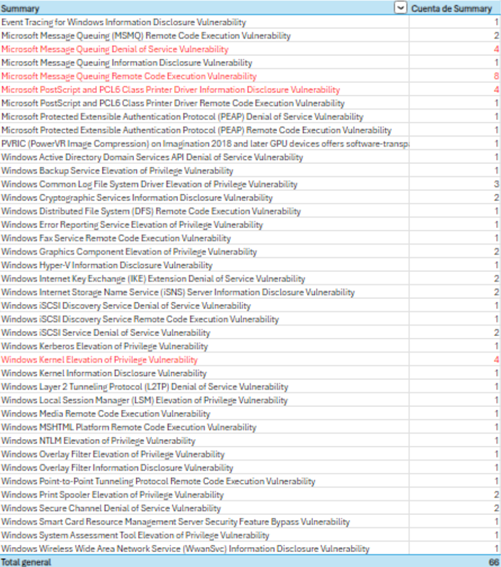
\includegraphics[width=0.3\linewidth]{ac11.png} % This is setting the figure to be .75x the width of the line. This can go all the way from 0.1 to 1 (and beyond, but then you're outside the page).
    \label{fig:OverallEffect}
\end{figure}

\subsection{Top de Vulnerabilidades Comunes} 

De acuerdo con la ocurrencia de las vulnerabilidades, en la tabla 1 se encuentra el top de vulnerabilidades.

\begin{table}[H]
    \caption{Top de vulnerabilidades para Windows 10 reportadas en 2023.}
    \centering
    \begin{tabular}{cc} %The c's here indicate the columns will be centered
        \hline 
         Tipo de Vulnerabilidades & Ocurrencia\\
         \hline
         Microsoft Message Queuing Remote Code Execution Vulnerability & 8\\
          Windows Kernel Elevation of Privilege Vulnerability & 4\\
	Microsoft PostScript and PCL6 Class Printer Driver Information Disclosure Vulnerability & 4\\
	Microsoft Message Queuing Denial of Service Vulnerability & 4\\
         \hline
    \end{tabular}
    \label{tab:table_words}
\end{table}

\subsection{Definición de las Vulnerabilidades en el Top} 

A continuación, se definen brevemente las 4 vulnerabilidades contempladas en el top:

\subsubsection{Microsoft Message Queuing Remote Code Execution Vulnerability}

Es una debilidad en el sistema de cola de mensajes de Microsoft Windows que podría permitir a un atacante ejecutar código de manera remota en un sistema afectado.

\subsubsection{Windows Kernel Elevation of Privilege Vulnerability}

Una vulnerabilidad de elevación de privilegios es cuando el kernel de Windows no logra manejar adecuadamente los objetos en memoria y un atacante puede aprovechar esta vulnerabilidad para ejecutar código arbitrario en modo kernel. El atacante podría entonces instalar programas, ver, cambiar, eliminar datos o cree nuevas cuentas con todos los derechos de usuario. Para aprovechar esta vulnerabilidad, un atacante primero tendría que iniciar sesión en el sistema y Luego el atacante podría ejecutar una aplicación especialmente diseñada para tomar el control de un sistema afectado. La actualización soluciona la vulnerabilidad corrigiendo la forma en que el kernel de Windows maneja los objetos en la memoria.

\subsubsection{Microsoft PostScript and PCL6 Class Printer Driver Information Disclosure Vulnerability}

La vulnerabilidad permite que un atacante remoto ejecute código arbitrario en el sistema. La vulnerabilidad existe debido a una validación insuficiente de la entrada proporcionada por el usuario en Microsoft PostScript y el controlador de impresora de clase PCL6. Un usuario remoto puede pasar entradas especialmente diseñadas a la aplicación y ejecutar código arbitrario en el sistema de destino.

\subsubsection{Microsoft Message Queuing Denial of Service Vulnerability}

Esta vulnerabilidad permite a un atacante enviar un mensaje especialmente diseñado a la cola de mensajes, lo que puede provocar una sobrecarga del sistema o un bloqueo del servicio MSMQ, lo que resulta en una denegación de servicio para los usuarios legítimos que intentan acceder a la cola de mensajes o utilizar servicios que dependen de ella.

\newpage

\section{\large Actividad 2 : Reporte de Instalación y virtualización de un sistema operativo de seguridad}

\subsection{¿Qué es VM?} 

Una máquina virtual (VM) es un entorno informático aislado con su propia CPU, memoria, interfaz de red y almacenamiento, creado a partir de recursos de hardware. También se puede definir como un software capaz de cargar en su interior otro sistema operativo haciéndole creer que es un PC de verdad, creando una máquina (PC, consola, móvil) que es virtual o emulada en vez de física. 

Con la virtualización es posible crear varias máquinas virtuales, cada una con su propio sistema operativo y aplicaciones dentro de una misma máquina física. Una máquina virtual no puede interactuar directamente con un sistema físico. En cambio, necesita una capa de software ligera, llamada hipervisor, para coordinarse con el hardware físico subyacente. El hipervisor asigna recursos informáticos físicos, como procesadores, memoria y almacenamiento, a cada máquina virtual. Mantiene cada máquina virtual separada de las otras para que no interfieran entre sí. 

\subsection{¿Cuál es la Utilidad de la Virtualización de Sistema Operativo? } 
La virtualización de sistema operativo permite la optimización en el uso de recursos, facilita la gestión y almacenamiento, mejora la seguridad y flexibilidad de los sistemas de TI. Sus principales utilidades son:
 
\begin{itemize}
\item  Consolidación de Servidores: ya que permite la ejecución de múltiples servidores en una sola máquina física, reduciendo el número de servidores necesarios. 
\item Aislamiento y Seguridad: ya que cada máquina virtual funciona de forma independiente, lo que aumenta la seguridad al aislar aplicaciones y procesos. 
\item Flexibilidad y Escalabilidad: ya que facilita la creación y eliminación de VMs según las necesidades, permitiendo una escalabilidad eficiente. 
\item Pruebas y Desarrollo: ya que proporciona entornos aislados para el desarrollo y pruebas de software, evitando conflictos con otros sistemas.
\item  Recuperación ante Desastres: ya que las VMs pueden ser fácilmente respaldadas y restauradas en diferentes hardware, mejorando así la capacidad de recuperación.
\end{itemize}

 \subsection{¿Qué es Kali Linux? }
 
 Kali Linux es una distribución de Linux basada en Debian que proporciona una amplia gama de herramientas de seguridad informática ya preinstaladas y listas para ejecutar. Entre estas herramientas se encuentran programas de escaneo de redes, análisis forense, pruebas de penetración, recopilación de información y herramientas de seguridad en general.  

\subsection{Instalación de Virtualizador }

Existen diversos softwares del hipervisor disponibles, sin embargo, para el desarrollo de esta actividad se seleccionó VirtualBox para la instalación.  

El sitio oficial de VirtualBox es el https://www.virtualbox.org \noindent \citep{virtualbox}\\

El equipo base en donde se instaló el VirtualBox, trabaja con Sistema Operativo Windows, por lo que descargó la versión “7.0.18” del siguiente enlace: \url{https://download.virtualbox.org/virtualbox/7.0.18/VirtualBox-7.0.18-162988-Win.exe }

\begin{figure}[H]
    \centering
    \caption{Sitio de VirtualBox para la descargar del instalador}
    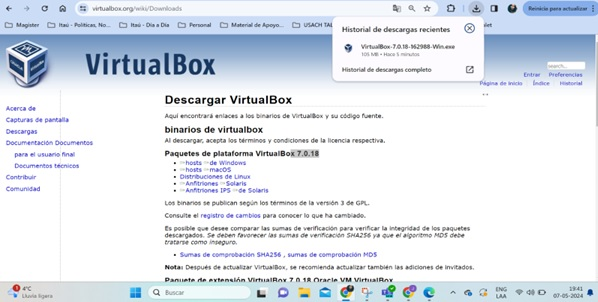
\includegraphics[width=0.6\linewidth]{imagenCap2/1.jpg} % This is setting the figure to be .75x the width of the line. This can go all the way from 0.1 to 1 (and beyond, but then you're outside the page).
    \label{fig:OverallEffect}
\end{figure}

Se ubica el archivo descargado y se ejecuta haciendo clic en el mismo. A continuación, se despliega el aplicativo para la instalación. 
Iniciamos el proceso, haciendo clic en el botón “Next”. Como se muestra en la Figura \ref{figura2.2}
\hfill \break

\begin{figure}[H]
    \centering
    \caption{Inicio de proceso de instalación.}
    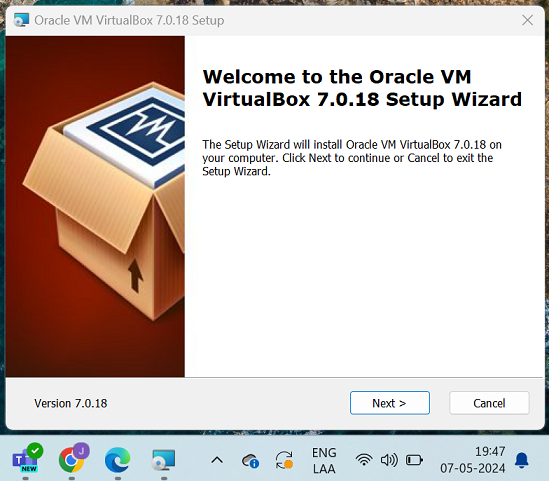
\includegraphics[width=0.5\linewidth]{imagenCap2/2.png} % This is setting the figure to be .75x the width of the line. This can go all the way from 0.1 to 1 (and beyond, but then you're outside the page).
    \label{figura2.2}
\end{figure}

\hfill \break
Luego de inicia el proceso de configuración personalizada de la máquina virtual, tal como árbol que instalará, aceptar advertencias del sistema y autorización para instalar dependencias faltantes.
\hfill \break
\begin{figure}[H]
    \centering
    \caption{Configuración personalizada – Árbol de instalación.}
    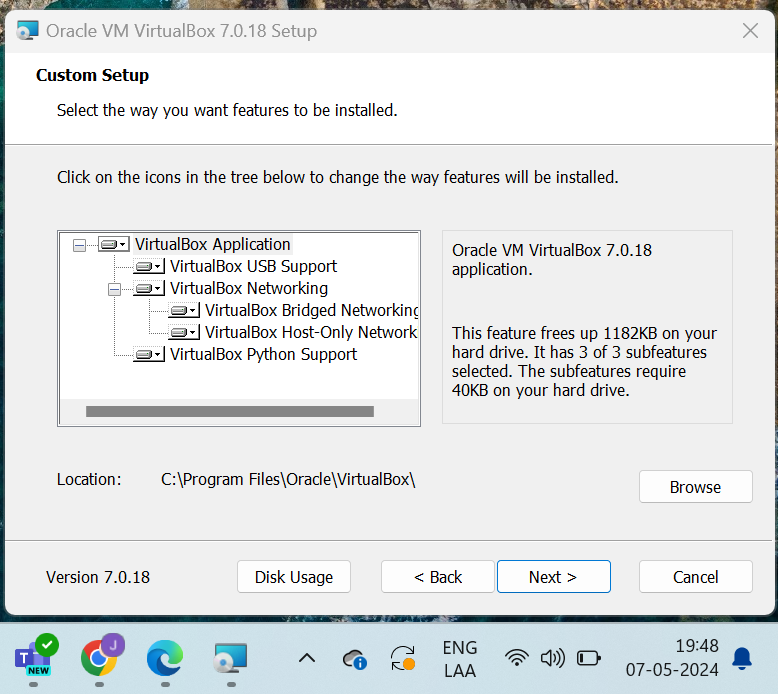
\includegraphics[width=0.5\linewidth]{imagenCap2/3.png} % This is setting the figure to be .75x the width of the line. This can go all the way from 0.1 to 1 (and beyond, but then you're outside the page).
    \label{fig:OverallEffect}
\end{figure}

 \hfill \break
\begin{figure}[H]
    \centering
    \caption{Configuración personalizada – Aceptar advertencia..}
    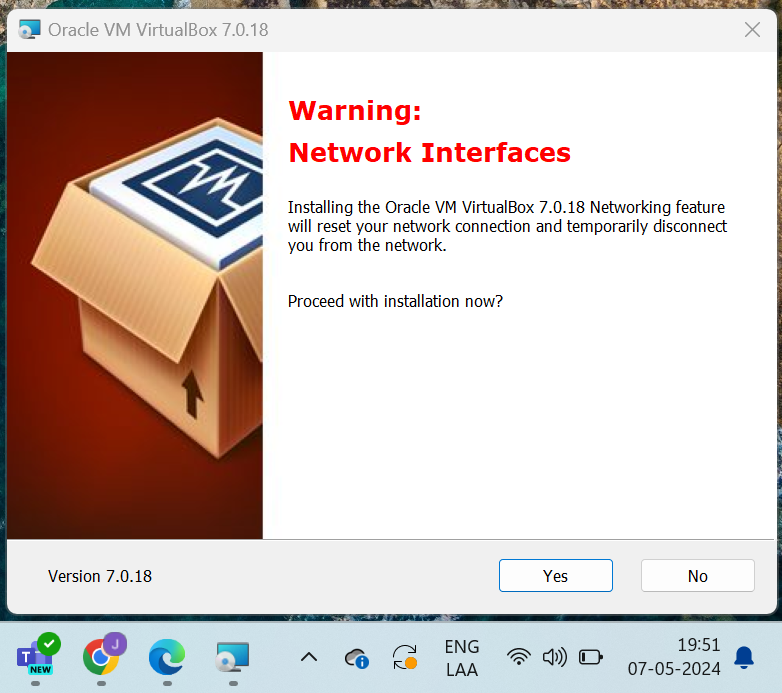
\includegraphics[width=0.5\linewidth]{imagenCap2/4.png} % This is setting the figure to be .75x the width of the line. This can go all the way from 0.1 to 1 (and beyond, but then you're outside the page).
    \label{fig:OverallEffect}
\end{figure}

 \hfill \break
\begin{figure}[H]
    \centering
    \caption{Configuración personalizada – Autorización para instalar dependencias faltantes.}
    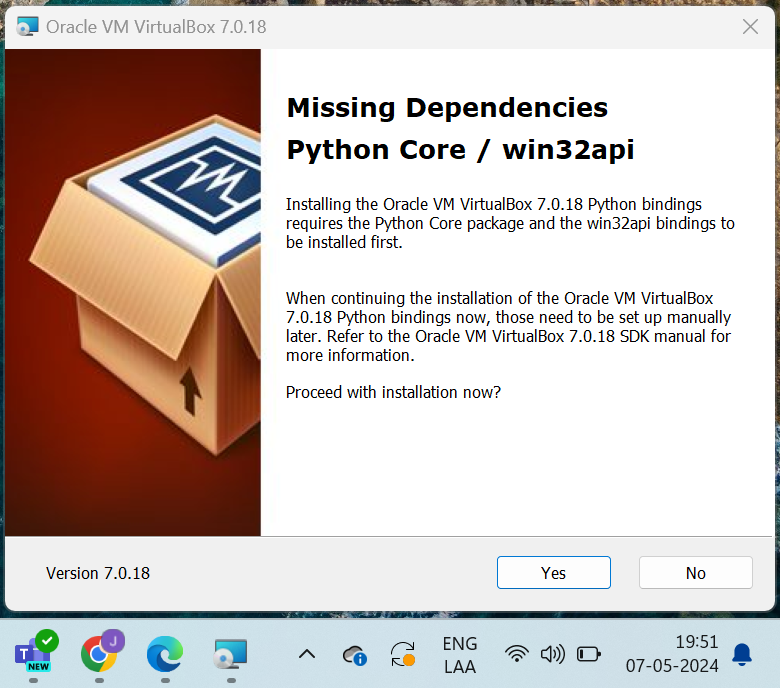
\includegraphics[width=0.5\linewidth]{imagenCap2/5.png} % This is setting the figure to be .75x the width of the line. This can go all the way from 0.1 to 1 (and beyond, but then you're outside the page).
    \label{fig:OverallEffect}
\end{figure}
\begin{figure}[H]
    \centering
    \caption{Iniciar la instalación personalizada.}
    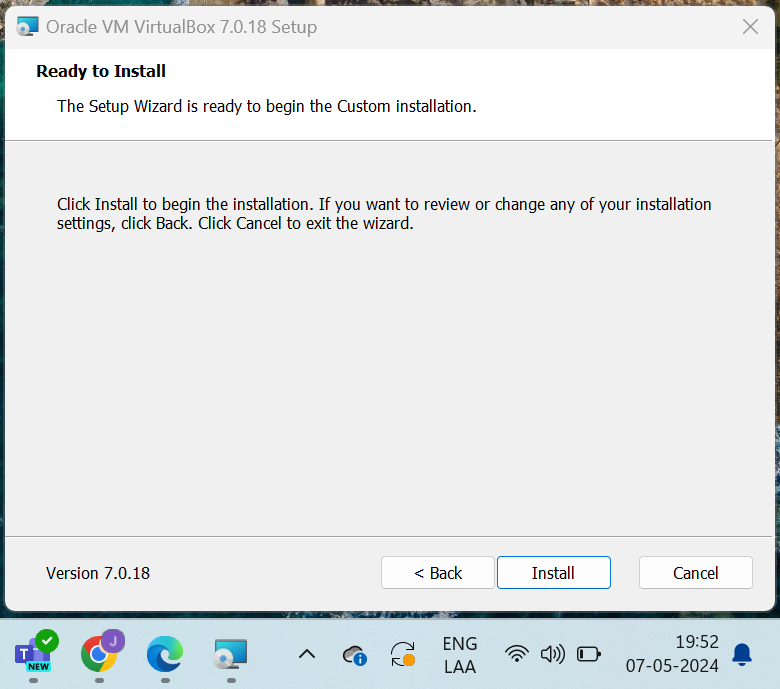
\includegraphics[width=0.5\linewidth]{imagenCap2/6.png} % This is setting the figure to be .75x the width of the line. This can go all the way from 0.1 to 1 (and beyond, but then you're outside the page).
    \label{fig:OverallEffect}
\end{figure}

Luego de iniciar la instalación y se muestra el estado de avance de esta.
\begin{figure}[H]
    \centering
    \caption{Vista para monitorear el estado de la instalación.}
    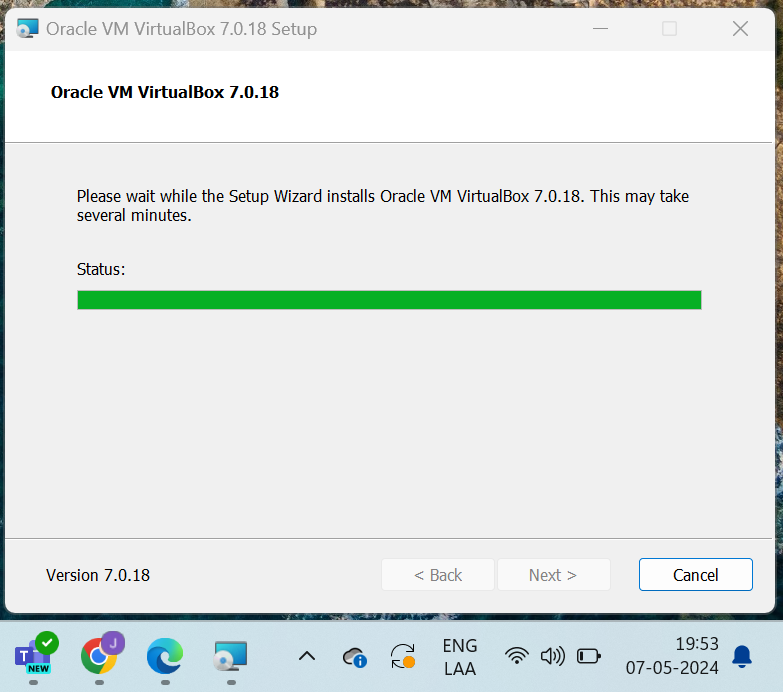
\includegraphics[width=0.5\linewidth]{imagenCap2/7.png} % This is setting the figure to be .75x the width of the line. This can go all the way from 0.1 to 1 (and beyond, but then you're outside the page).
    \label{fig:OverallEffect}
\end{figure}

\begin{figure}[H]
    \centering
    \caption{Finalizar la instalación.}
    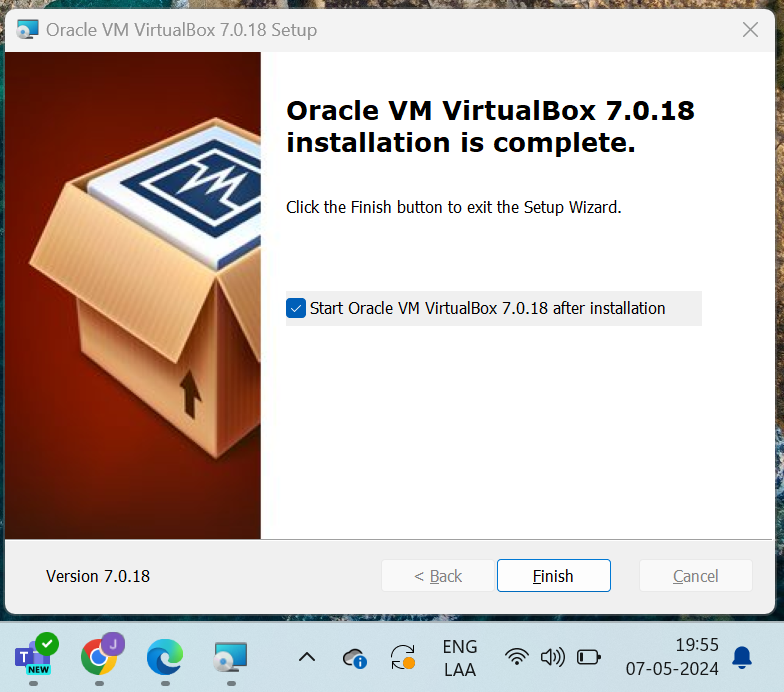
\includegraphics[width=0.5\linewidth]{imagenCap2/8.png} % This is setting the figure to be .75x the width of the line. This can go all the way from 0.1 to 1 (and beyond, but then you're outside the page).
    \label{fig:OverallEffect}
\end{figure}

Finalmente, la máquina virtual se encontrará instalada y lista para realizar las virtualizaciones requeridas según las actividades posteriores a desarrollar.
 \hfill \break
\begin{figure}[H]
    \centering
    \caption{Máquina Virtual ya instalada - Vista principal de VirtualBox.}
    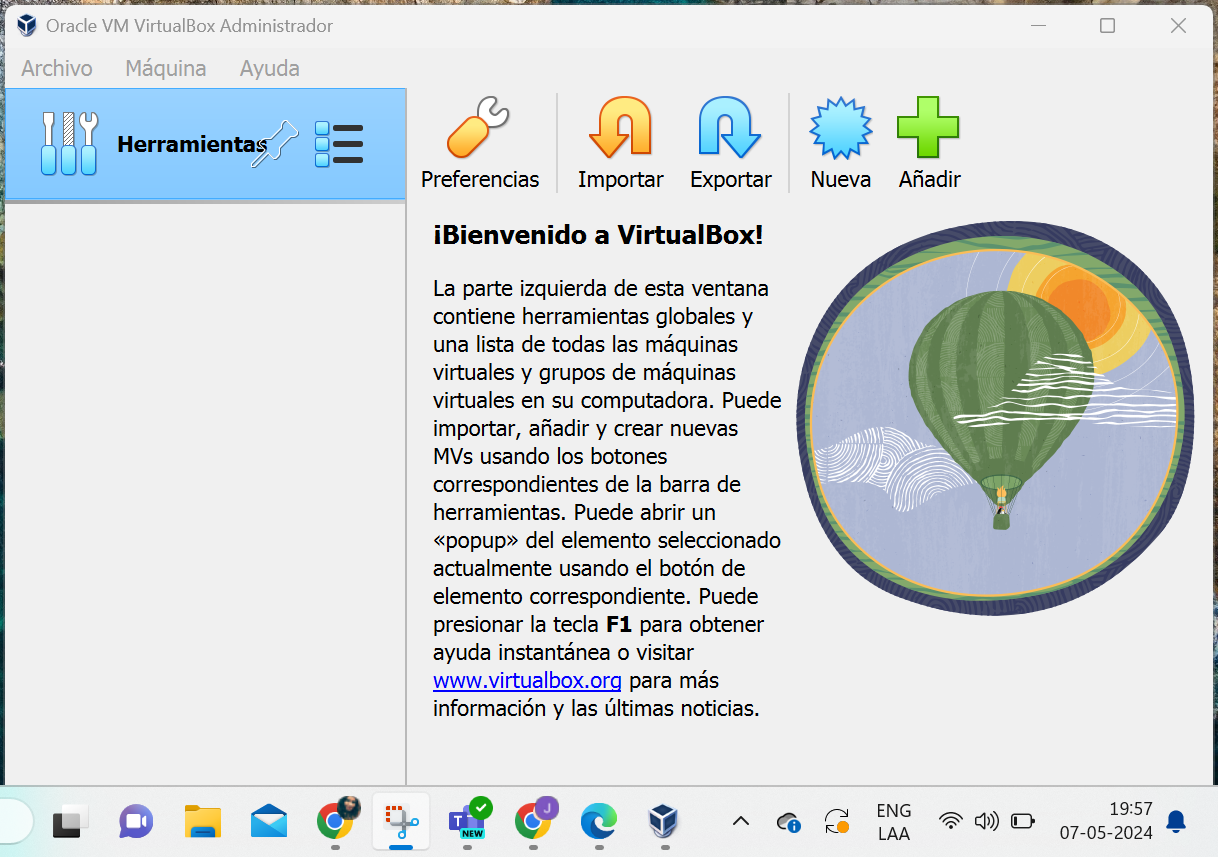
\includegraphics[width=0.5\linewidth]{imagenCap2/9.png} % This is setting the figure to be .75x the width of the line. This can go all the way from 0.1 to 1 (and beyond, but then you're outside the page).
    \label{fig:OverallEffect}
\end{figure}
 
\subsection{Instalación de Sistema Operativo Virtualizado}

A continuación, se procede a la descarga de la imagen del sistema operativo seleccionado para el desarrollo de esta actividad, el cual es Kali Linux, el sitio oficial de este es el \url{https://www.kali.org}.  \citep{kali}

\begin{figure}[H]
    \centering
    \caption{Sitio Oficial Kali Linux.}
    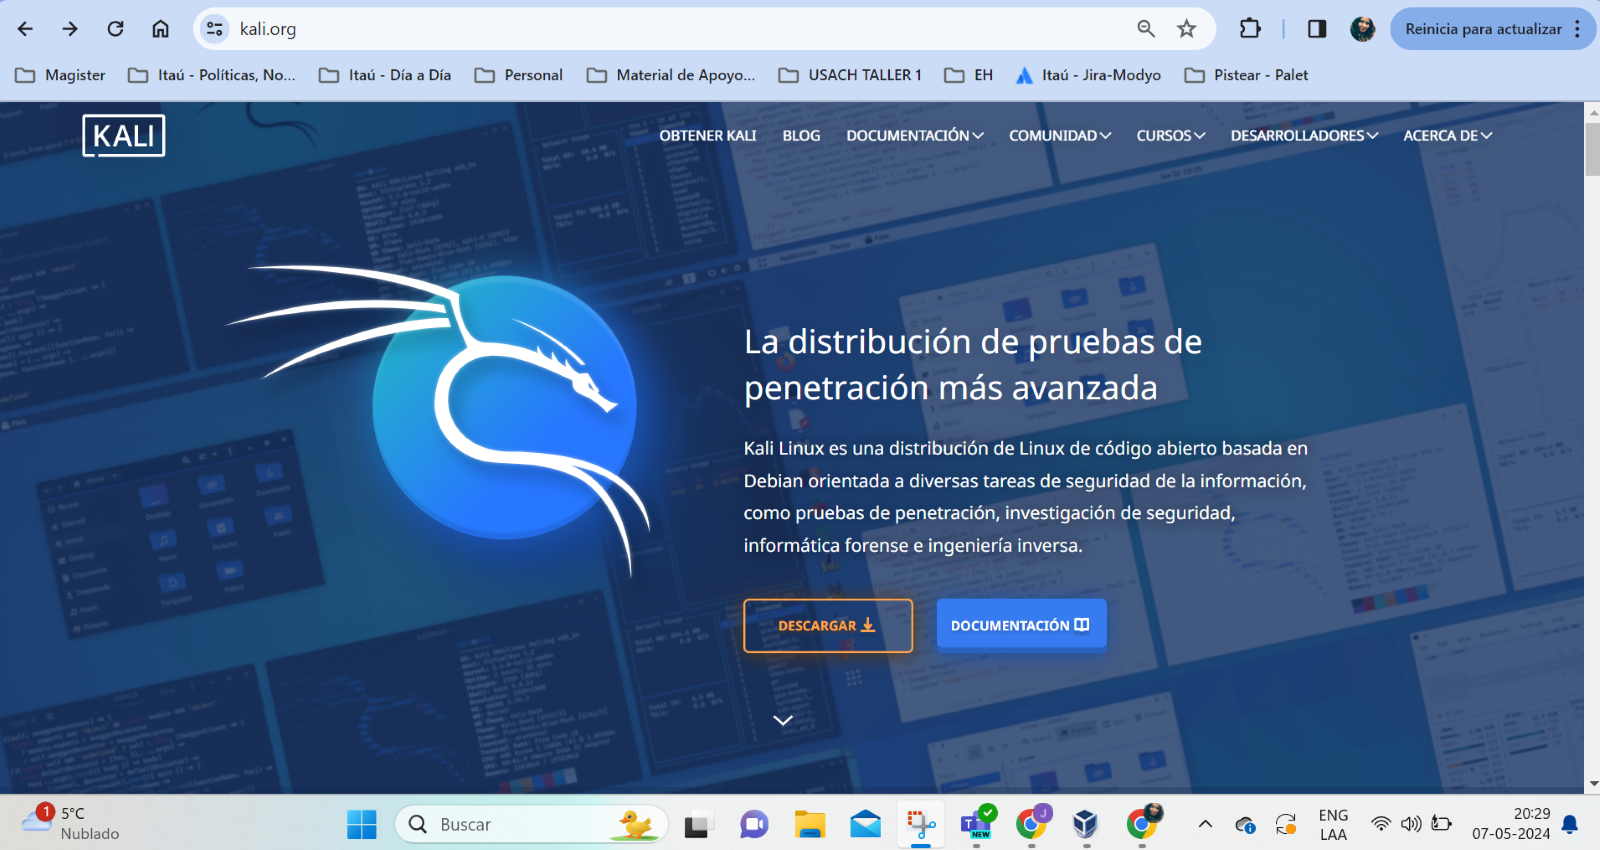
\includegraphics[width=0.5\linewidth]{imagenCap2/10.png} % This is setting the figure to be .75x the width of the line. This can go all the way from 0.1 to 1 (and beyond, but then you're outside the page).
    \label{fig:OverallEffect}
\end{figure}

Para descargar Kali Linux, debe hacer clic en el botón de “Descarga”, lo cual conduce a \url{https://www.kali.org/get-kali/#kali-platforms} en donde se debe seleccionar la descarga relacionada a “Imágenes del Instalador”.

A continuación, se debe seleccionar que tipo Sistema (respecto a los bits) se posee en el equipo base donde se realizará la instalación. En este caso 64bits para VirtualBox.

\begin{figure}[H]
    \centering
    \caption{Sitio oficial de Kali Linux - Descarga de imagen del instalador según bits de equipo base.}
    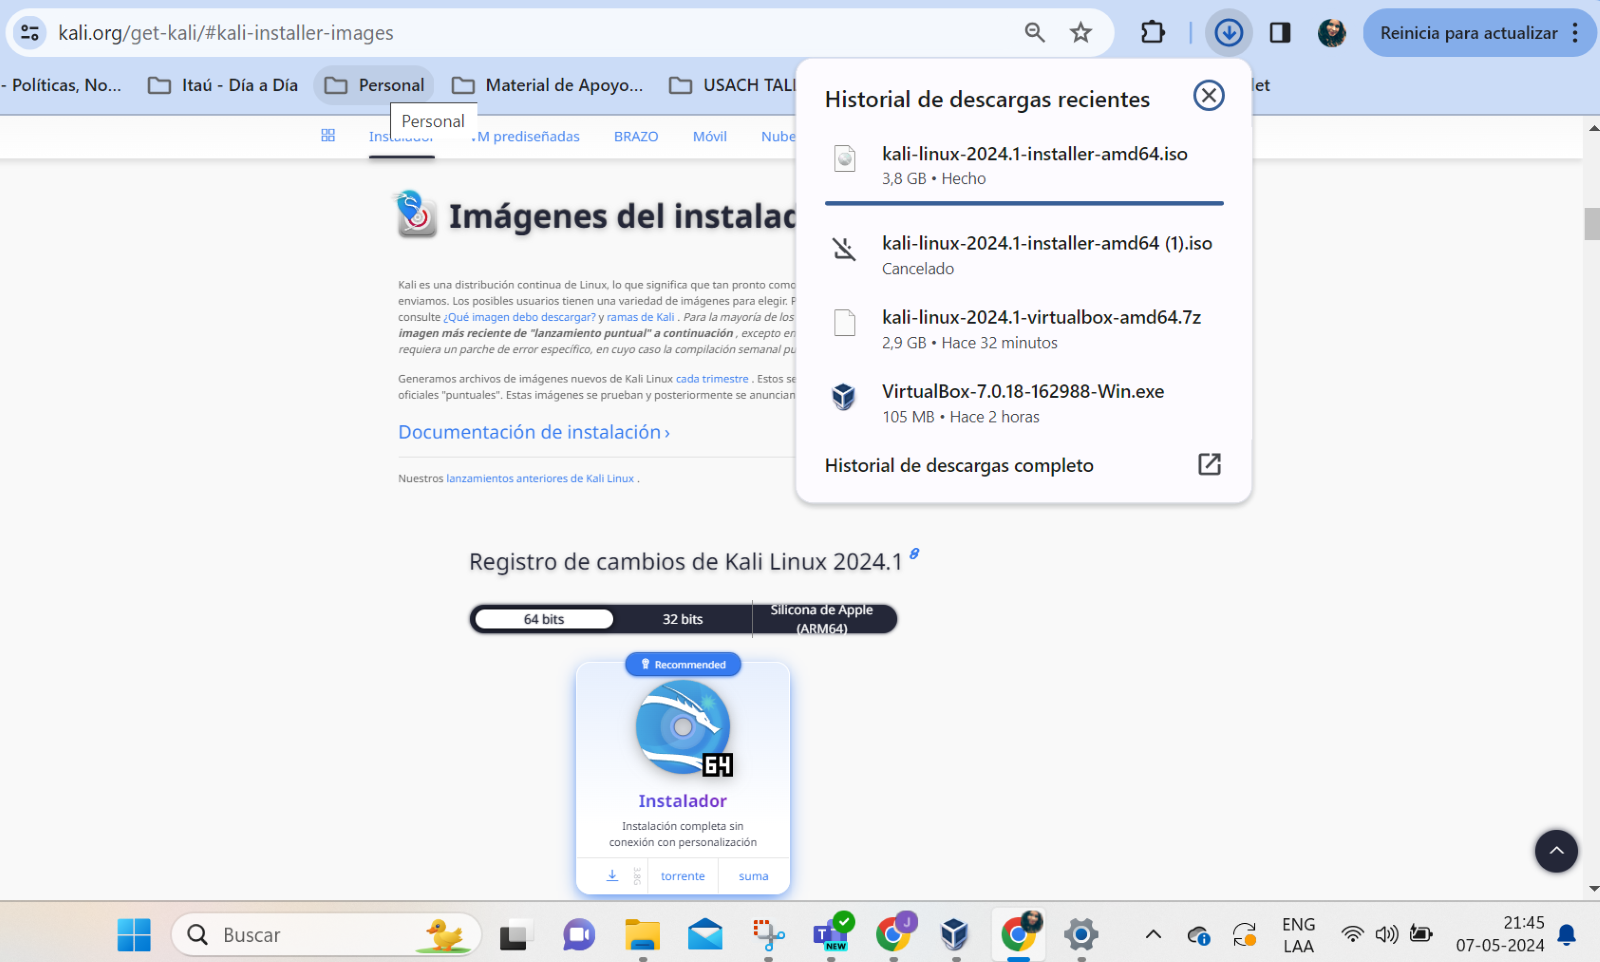
\includegraphics[width=0.5\linewidth]{imagenCap2/11.png} % This is setting the figure to be .75x the width of the line. This can go all the way from 0.1 to 1 (and beyond, but then you're outside the page).
    \label{fig:OverallEffect}
\end{figure}

Luego de contar con la imagen, se procede a crear una máquina virtual nueva en VirtualBox, haciendo uso de la opción “Añadir”.

\begin{figure}[H]
    \centering
    \caption{VirtualBox - Añadir nueva máquina virtual.}
    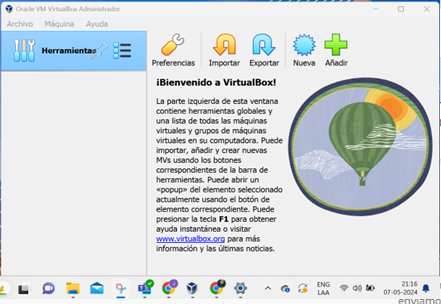
\includegraphics[width=0.5\linewidth]{imagenCap2/12.png} % This is setting the figure to be .75x the width of the line. This can go all the way from 0.1 to 1 (and beyond, but then you're outside the page).
    \label{fig:OverallEffect}
\end{figure}

Se inicia la creación de la máquina virtual, se establece el nombre, se le asigna una ruta, se le suministra la ruta de la .iso a instalar, se la asigna RAM y número de CPU virtuales, así como se crea y asigna capacidad a un disco duro virtual (también se puede asignar un disco duro existente).

\begin{figure}[H]
    \centering
    \caption{Configuración de Máquina Virtual – Nombre y sistema operativo.}
    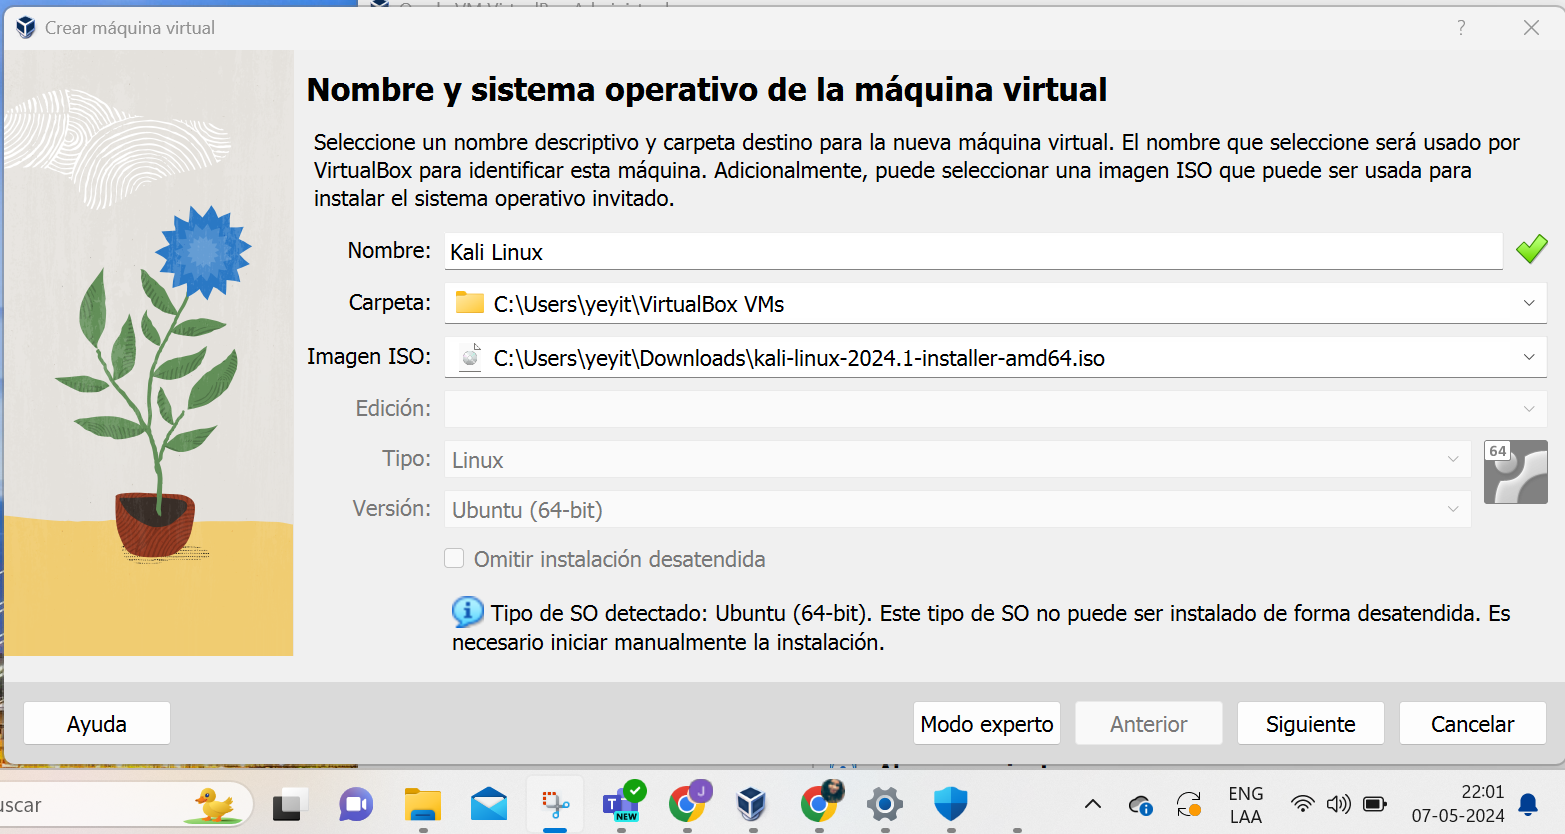
\includegraphics[width=0.5\linewidth]{imagenCap2/13.png} % This is setting the figure to be .75x the width of the line. This can go all the way from 0.1 to 1 (and beyond, but then you're outside the page).
    \label{fig:OverallEffect}
\end{figure}

\begin{figure}[H]
    \centering
    \caption{Configuración de Máquina Virtual – RAM y CPU virtuales.}
    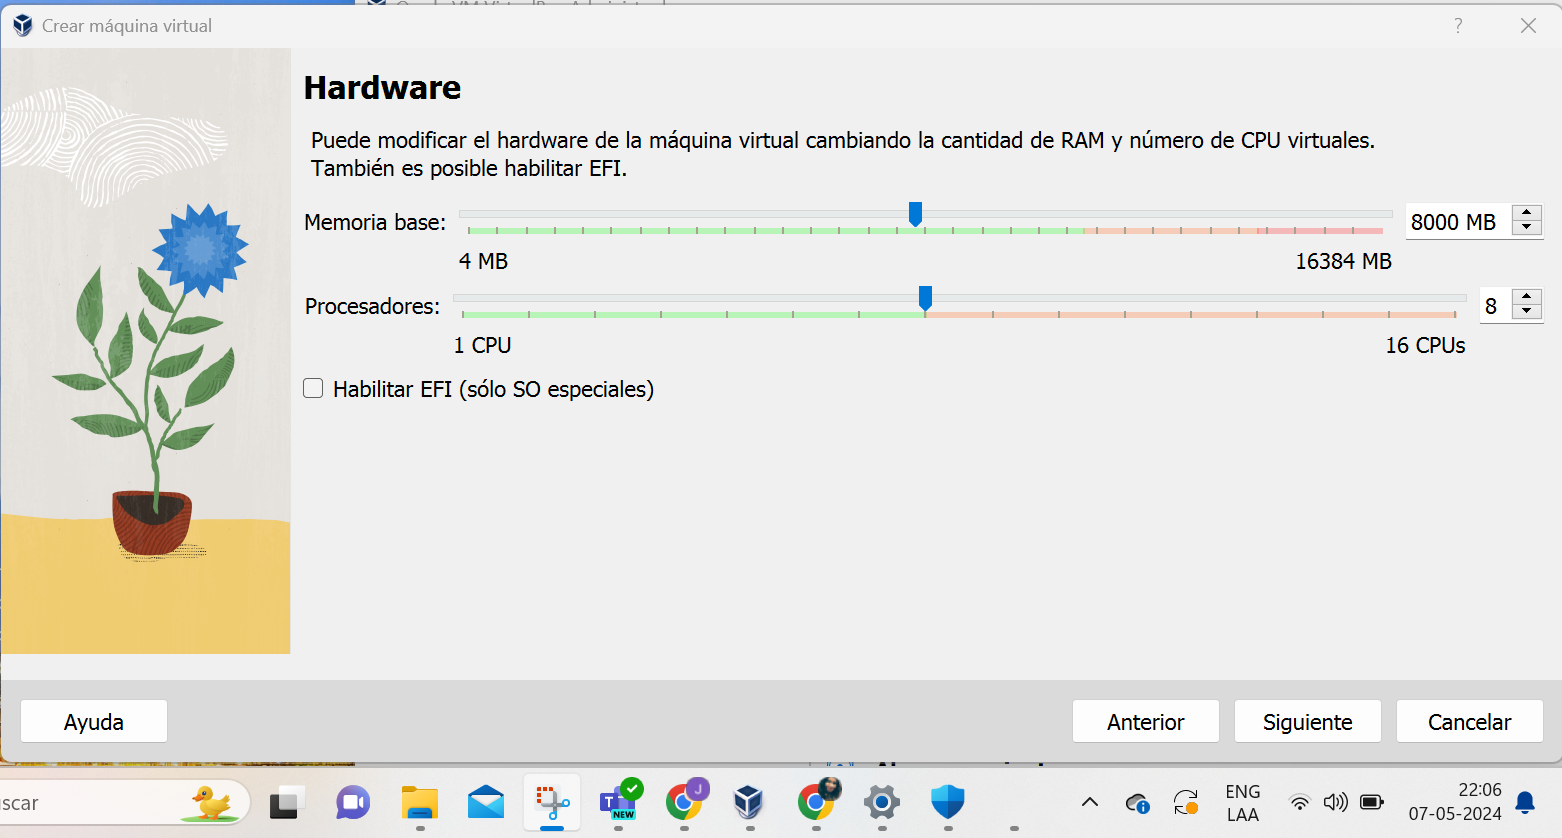
\includegraphics[width=0.5\linewidth]{imagenCap2/14.png} % This is setting the figure to be .75x the width of the line. This can go all the way from 0.1 to 1 (and beyond, but then you're outside the page).
    \label{fig:OverallEffect}
\end{figure}

\begin{figure}[H]
    \centering
    \caption{Configuración de Máquina Virtual – Disco Duro Virtual.}
    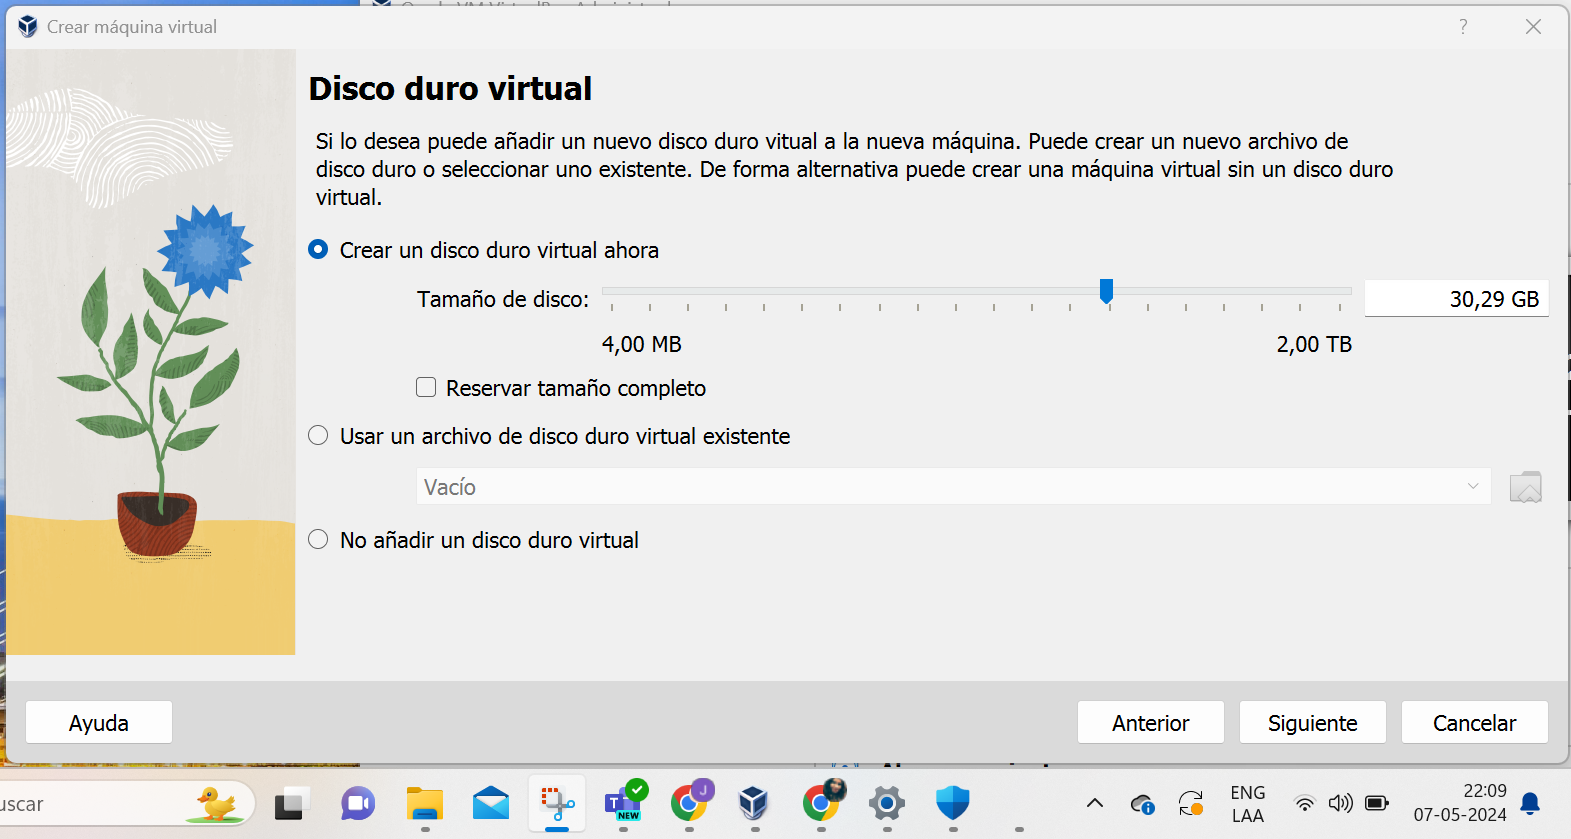
\includegraphics[width=0.5\linewidth]{imagenCap2/15.png} % This is setting the figure to be .75x the width of the line. This can go all the way from 0.1 to 1 (and beyond, but then you're outside the page).
    \label{fig:OverallEffect}
\end{figure}

\begin{figure}[H]
    \centering
    \caption{Configuración de Máquina Virtual – Resumen de configuración.}
    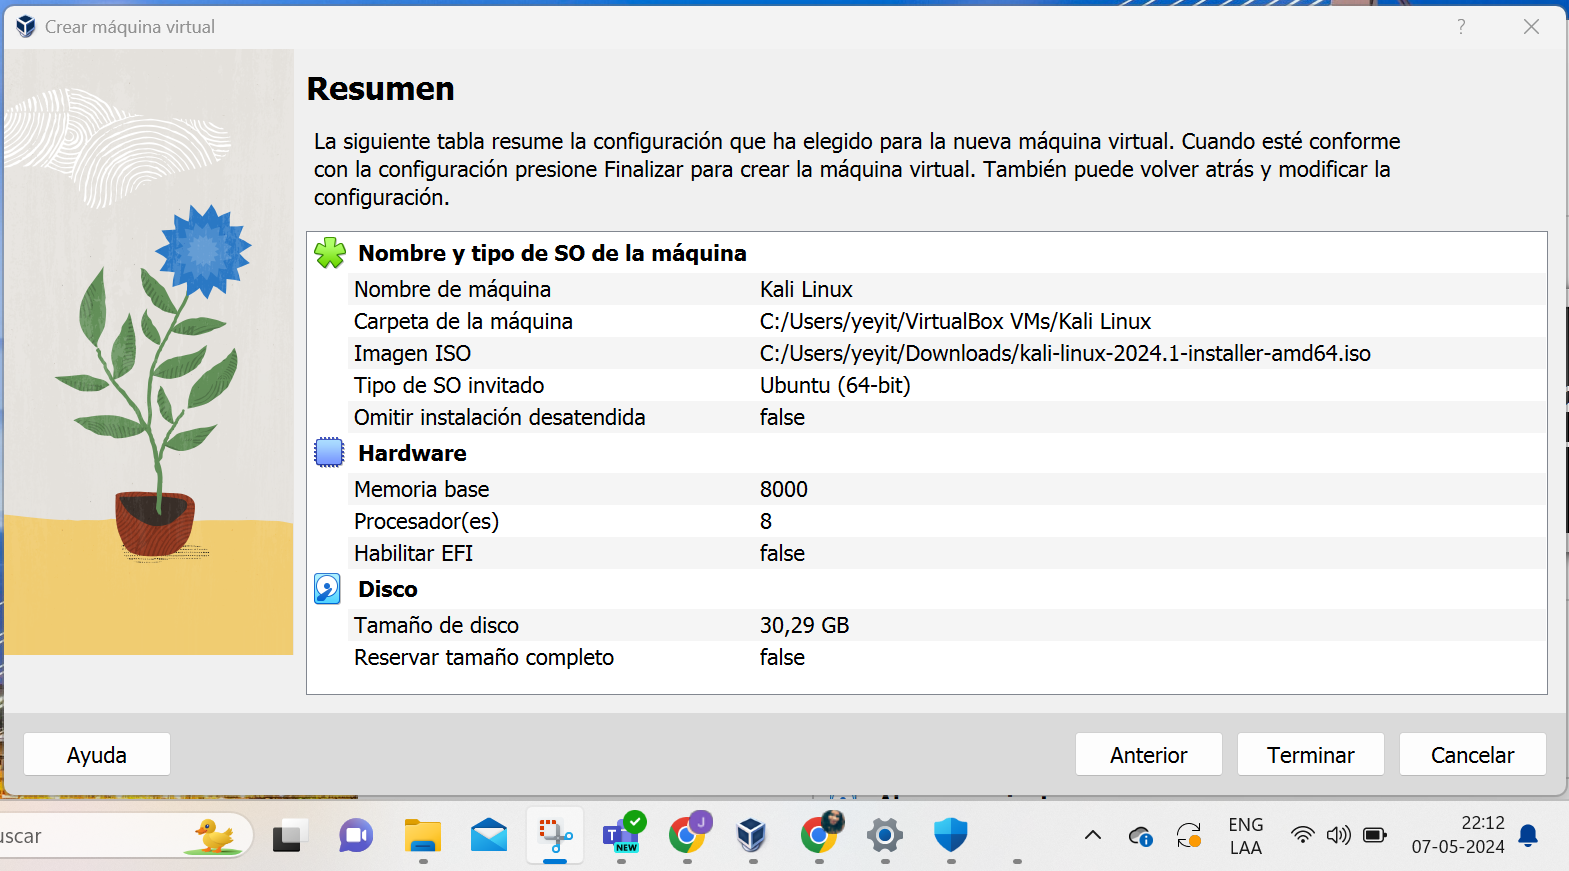
\includegraphics[width=0.5\linewidth]{imagenCap2/16.png} % This is setting the figure to be .75x the width of the line. This can go all the way from 0.1 to 1 (and beyond, but then you're outside the page).
    \label{fig:OverallEffect}
\end{figure}

\subsection{Configuración de Sistema Operativo – Kali Linux}

Ya creada la máquina virtual Kali Linux, se selecciona e inicia para realizar las configuraciones de esta, a nivel de idioma, red, usuario y contraseña, particionado de disco, cargador de arranque.

\begin{figure}[H]
    \centering
    \caption{Iniciar Máquina Virtual Kali Linux.}
    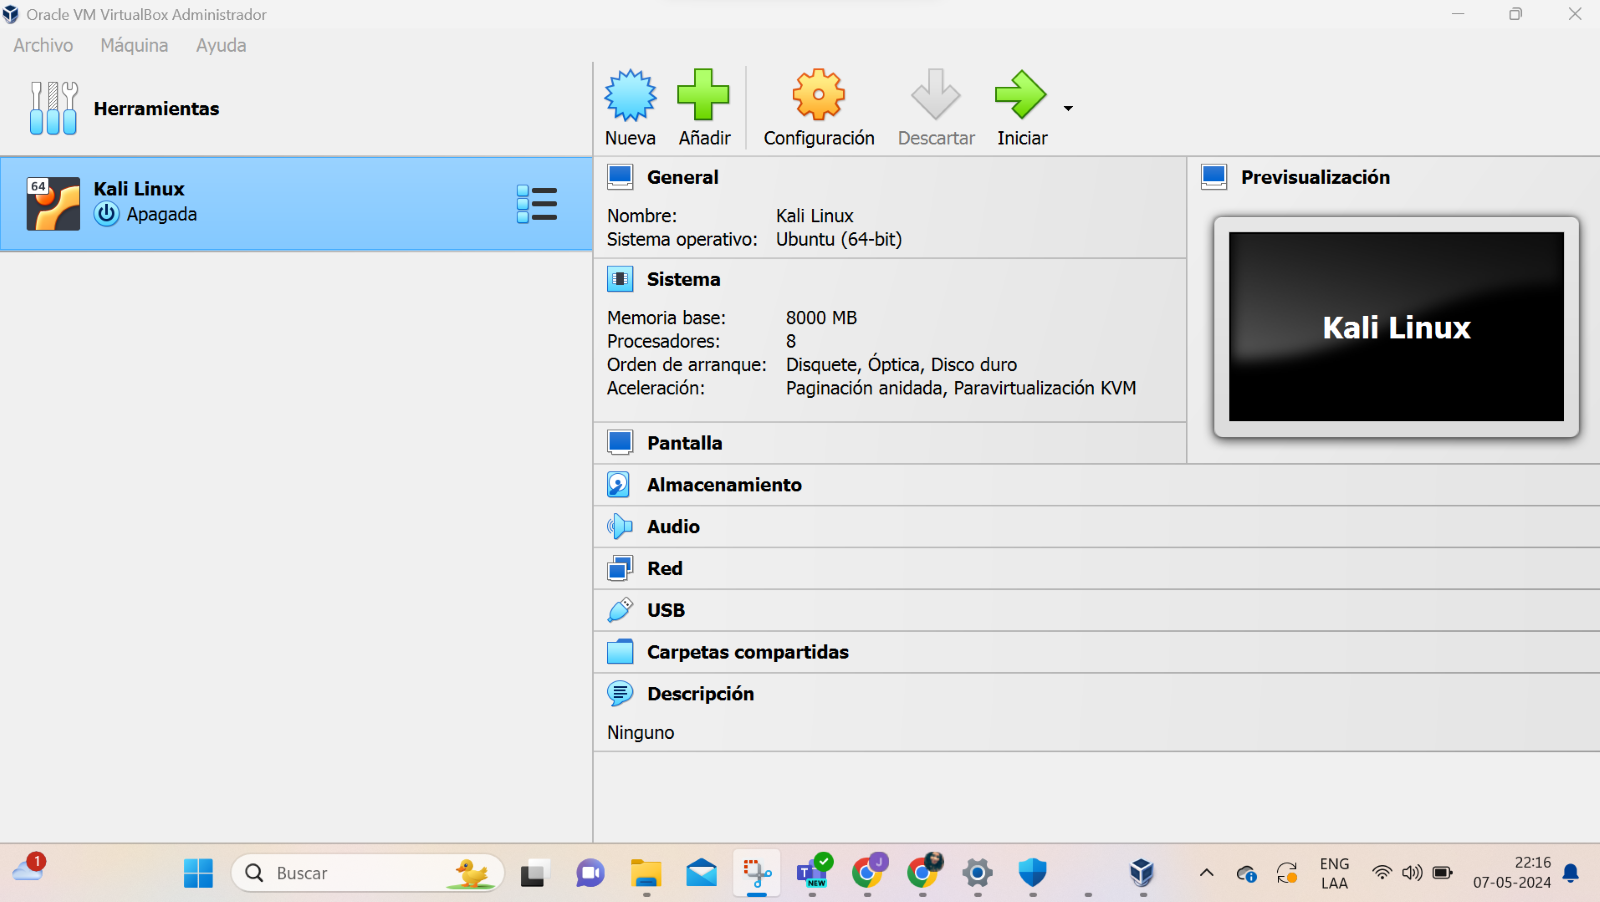
\includegraphics[width=0.5\linewidth]{imagenCap2/17.png} % This is setting the figure to be .75x the width of the line. This can go all the way from 0.1 to 1 (and beyond, but then you're outside the page).
    \label{fig:OverallEffect}
\end{figure}

\begin{figure}[H]
    \centering
    \caption{Configuración Kali Linux - Idioma.}
    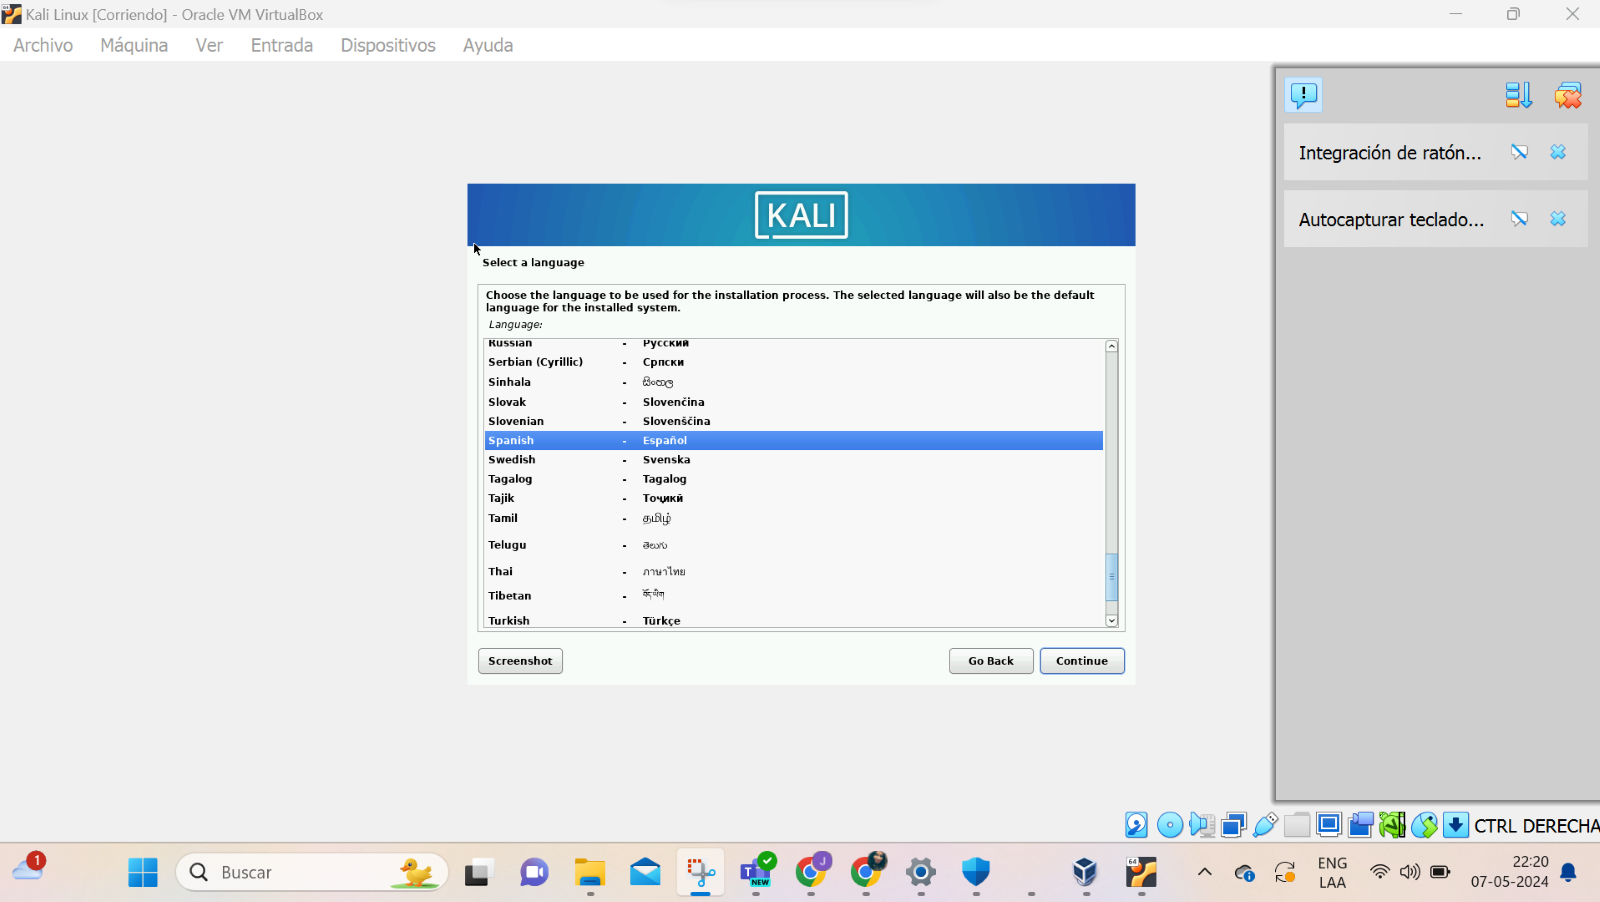
\includegraphics[width=0.5\linewidth]{imagenCap2/18.png} % This is setting the figure to be .75x the width of the line. This can go all the way from 0.1 to 1 (and beyond, but then you're outside the page).
    \label{fig:OverallEffect}
\end{figure}

\begin{figure}[H]
    \centering
    \caption{Configuración Kali Linux - Red.}
    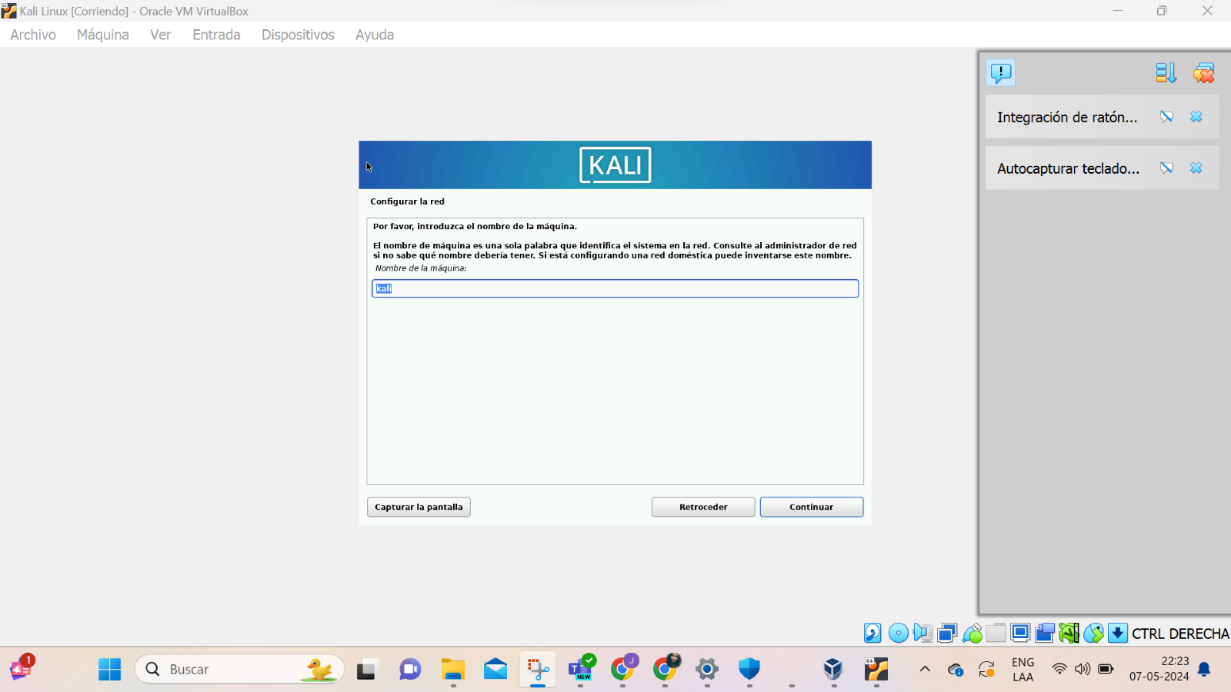
\includegraphics[width=0.5\linewidth]{imagenCap2/19.png} % This is setting the figure to be .75x the width of the line. This can go all the way from 0.1 to 1 (and beyond, but then you're outside the page).
    \label{fig:OverallEffect}
\end{figure}

\begin{figure}[H]
    \centering
    \caption{Configuración Kali Linux - Usuario.}
    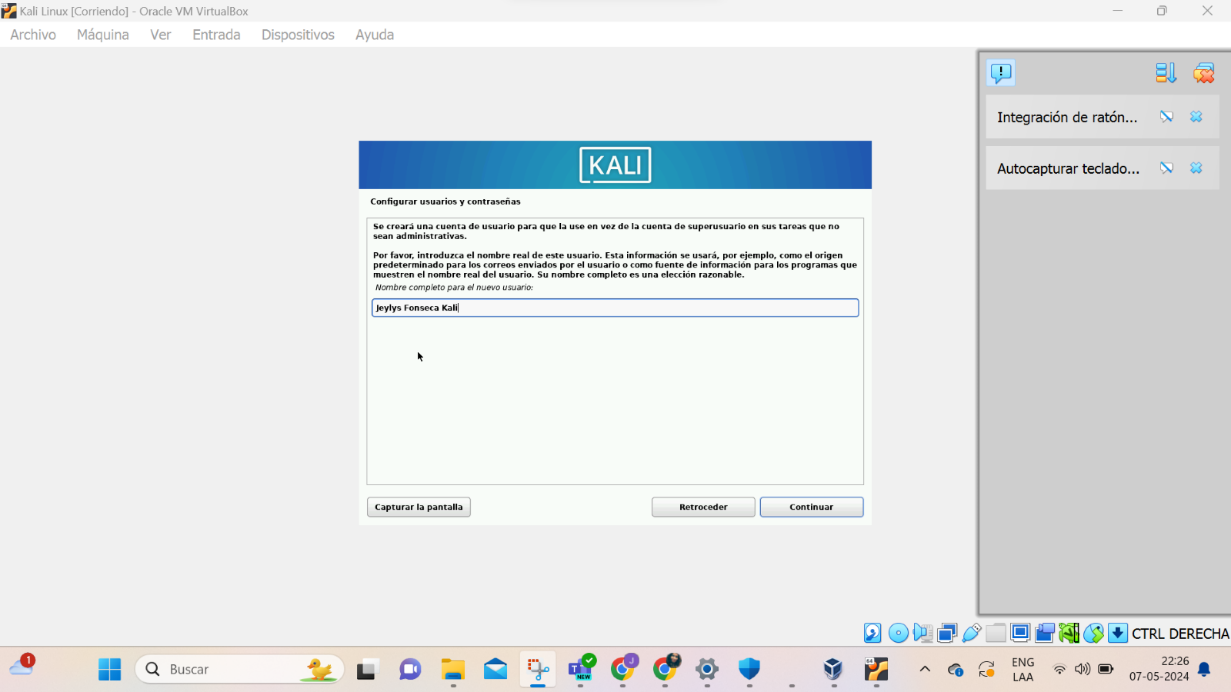
\includegraphics[width=0.5\linewidth]{imagenCap2/20.png} % This is setting the figure to be .75x the width of the line. This can go all the way from 0.1 to 1 (and beyond, but then you're outside the page).
    \label{fig:OverallEffect}
\end{figure}

\begin{figure}[H]
    \centering
    \caption{Configuración Kali Linux - Contraseña.}
    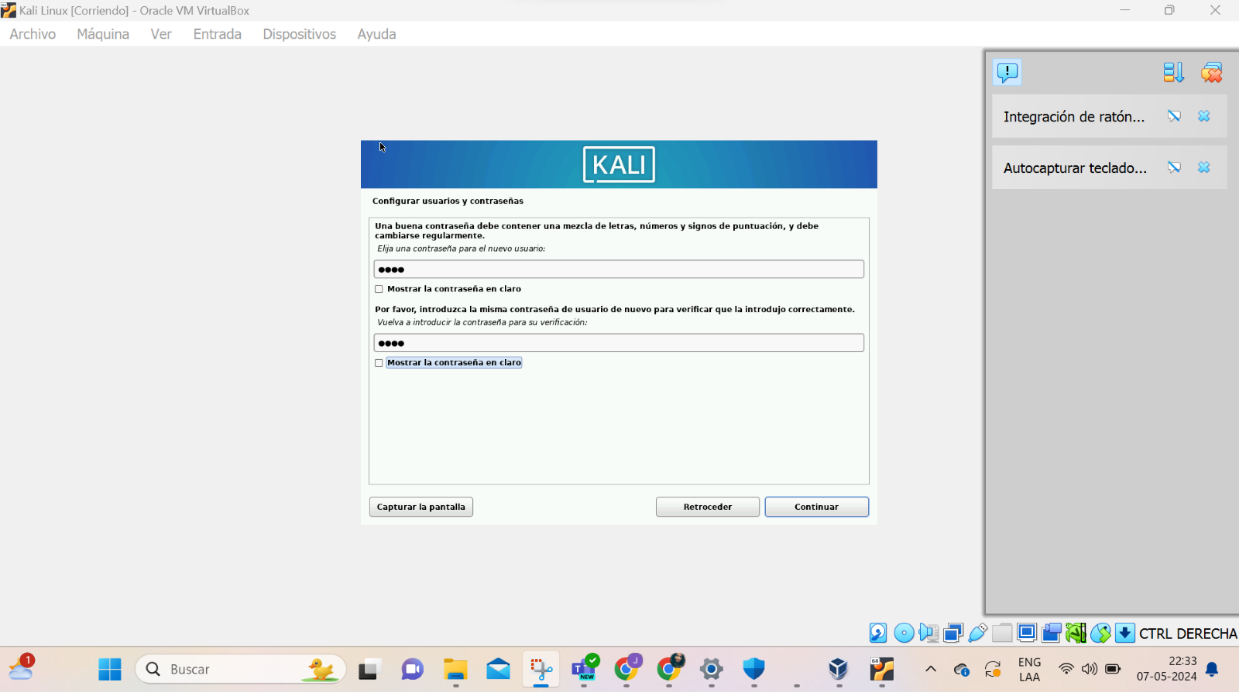
\includegraphics[width=0.5\linewidth]{imagenCap2/21.png} % This is setting the figure to be .75x the width of the line. This can go all the way from 0.1 to 1 (and beyond, but then you're outside the page).
    \label{fig:OverallEffect}
\end{figure}

\begin{figure}[H]
    \centering
    \caption{Configuración Kali Linux – Resumen y finalizado de particionado de disco.}
    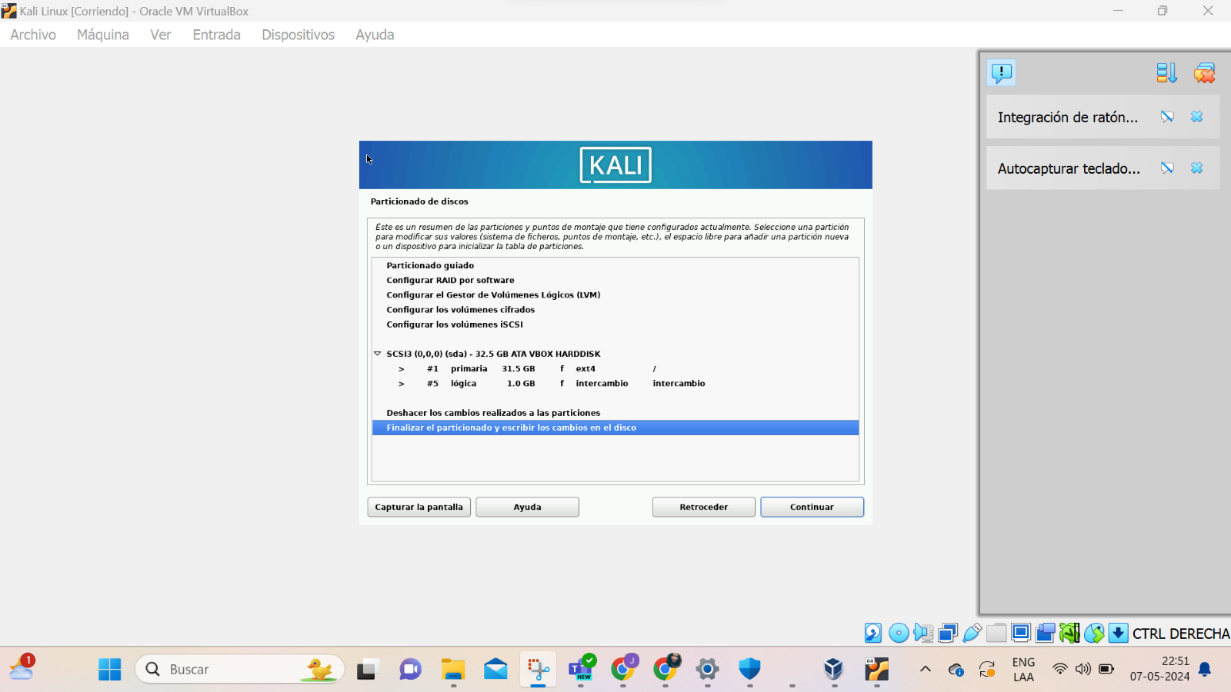
\includegraphics[width=0.5\linewidth]{imagenCap2/22.png} % This is setting the figure to be .75x the width of the line. This can go all the way from 0.1 to 1 (and beyond, but then you're outside the page).
    \label{fig:OverallEffect}
\end{figure}

\begin{figure}[H]
    \centering
    \caption{Configuración Kali Linux – Cargador de Arranque}
    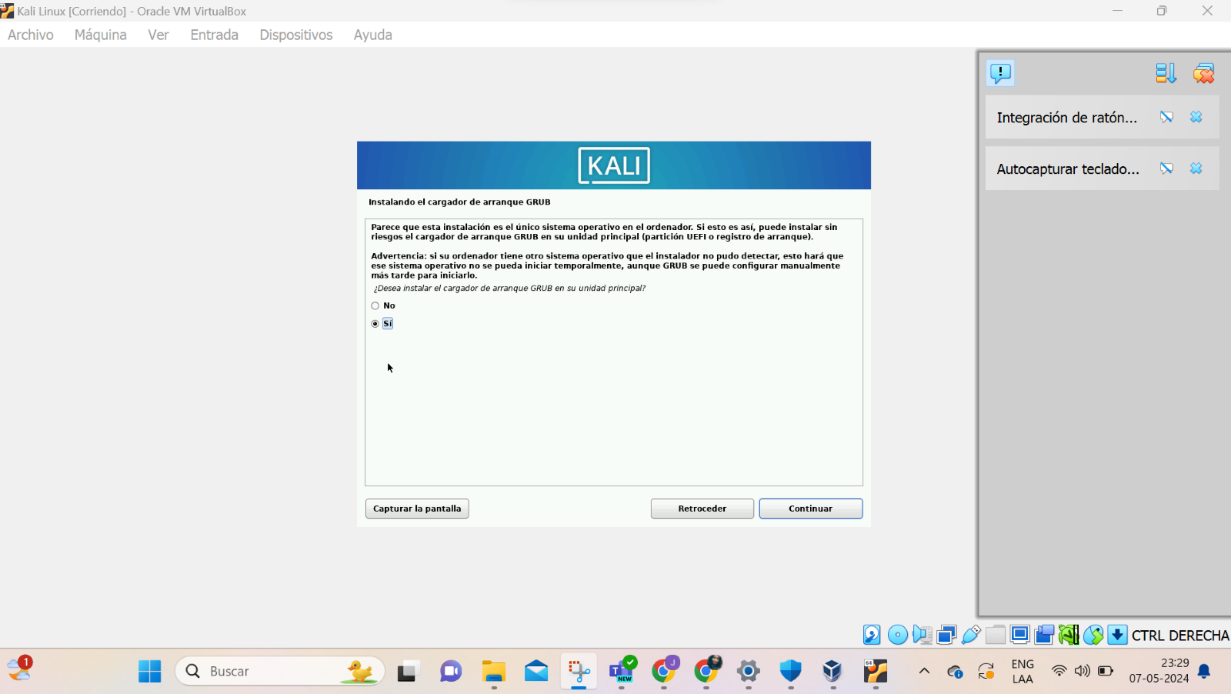
\includegraphics[width=0.5\linewidth]{imagenCap2/23.png} % This is setting the figure to be .75x the width of the line. This can go all the way from 0.1 to 1 (and beyond, but then you're outside the page).
    \label{fig:OverallEffect}
\end{figure}

\begin{figure}[H]
    \centering
    \caption{Kali Linux Instalado, configurado, en ejecución e iniciado sesión.}
    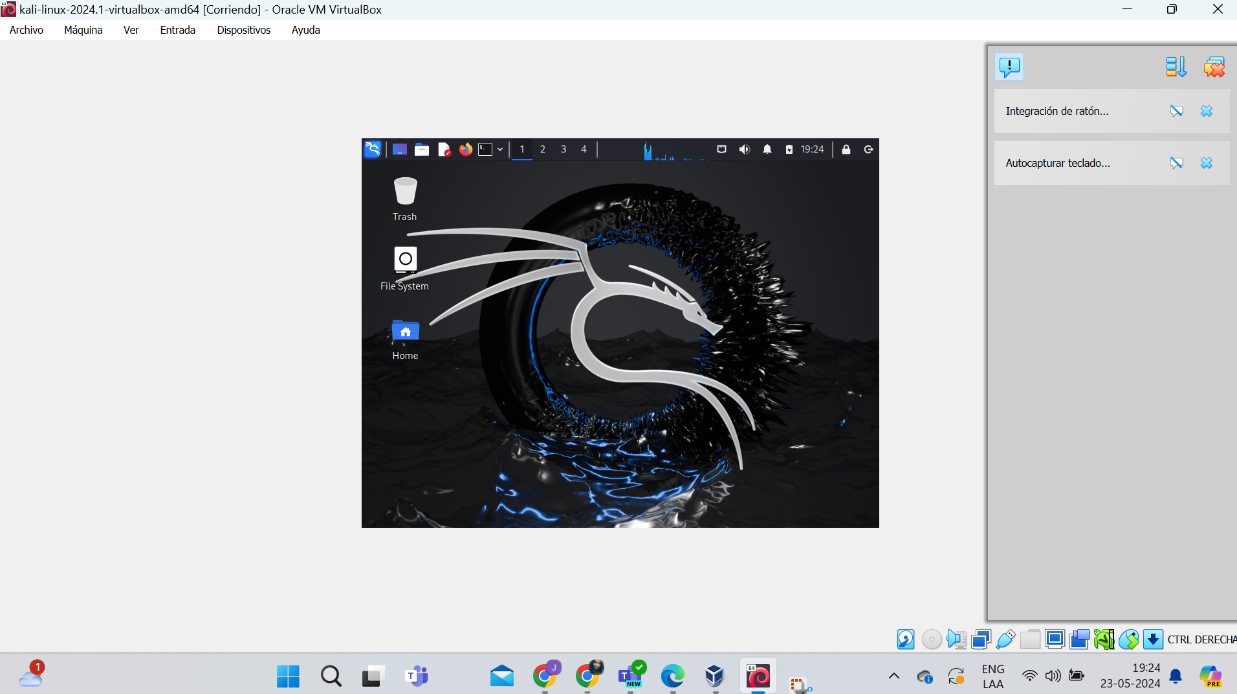
\includegraphics[width=0.5\linewidth]{imagenCap2/24.png} % This is setting the figure to be .75x the width of the line. This can go all the way from 0.1 to 1 (and beyond, but then you're outside the page).
    \label{fig:OverallEffect}
\end{figure}

\subsection{Análisis - Uso de Kali Linux Virtualizado}

Es esencial para ingenieros de ciberseguridad disponer de un sistema operativo como Kali Linux de forma virtualizada, ya que proporciona un entorno además de seguro, aislado para realizar pruebas sin afectar el sistema anfitrión. La capacidad de recuperación rápida y portabilidad, facilitan la movilidad y la eficiencia en las actividades cotidianas de los colaboradores en ciberseguridad. Con este tipo de sistemas operativos virtualizados, se optimiza el consumo de recursos, permite probar distintas configuraciones y mejora la seguridad en general al contener actividades que podrían ser dañinas en un entorno controlado. La virtualización de Kali Linux, en resumen, es crucial para el desarrollo de actividades en ciberseguridad, ofreciendo flexibilidad, seguridad y eficiencia.
 


\newpage

\section{\large Actividad 3}
%\noindent \maskCitet{cervantes1999}\\

\subsection{¿Qué es Docker?} 
Permite a los desarrolladores a crear, compartir, ejecutar y verificar aplicaciones en cualquier lugar, sin necesidad de tediosa configuración o administración del entorno. 
\noindent \maskCitet{docker}\\

Para esta actividad a los alumnos se les facilito el uso de las opciones de ejecutar docker desde un entorno local de pruebas por medio de la instalación en una maquina local o por medio del uso de play with docker.

En esta oportunidad se escogió la herramienta play with docker \noindent\maskCitet{playwithdocker}\\ la cual es una herramienta de uso gratuito por la que el usuario puede hacer uso de hasta 5 instancias en paralelo por 4 horas de sesión.

\subsection{Uso de Docker} 

Para poder realizar el uso de esta aplicación solo es necesario tener una cuenta con cualquier correo electrónico en docker. Una vez autenticados la página nos da la opción de iniciar mediante el botón Start.

\begin{figure}[H]
    \centering
    \caption{Logo de Docker.}
    
\includegraphics[width=0.3\linewidth]{docker1.png} % This is setting the figure to be .75x the width of the line. This can go all the way from 0.1 to 1 (and beyond, but then you're outside the page).
    \label{fig:OverallEffect}
\end{figure}

Una vez dentro de la página principal tenemos al lado izquierdo superior el contador que comienza a contar en cuenta regresiva las 4 horas de uso de las instancias. Para esta actividad solo usaremos la opción de +ADD NEW INSTANCE. La que al pinchar nos abrirá una instancia con docker ya instalado. 

\begin{figure}[H]
    \centering
    \caption{Inicio de instancia en play with Docker}
    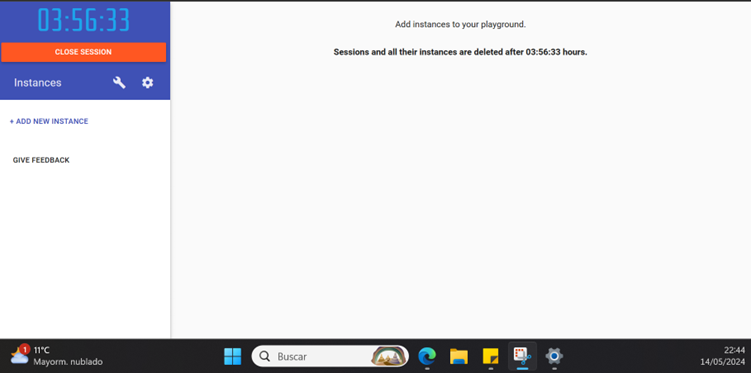
\includegraphics[width=0.75\linewidth]{docker2.png} % This is setting the figure to be .75x the width of the line. This can go all the way from 0.1 to 1 (and beyond, but then you're outside the page).
    \label{fig:OverallEffect}
\end{figure}

Para verificar que docker está instalado en la instancia debemos ingresar el comando docker –version y se mostrara por la consola de la instancia la versión instalada de docker.

\begin{figure}[H]
    \centering
    \caption{Consola de play with Docker.}
    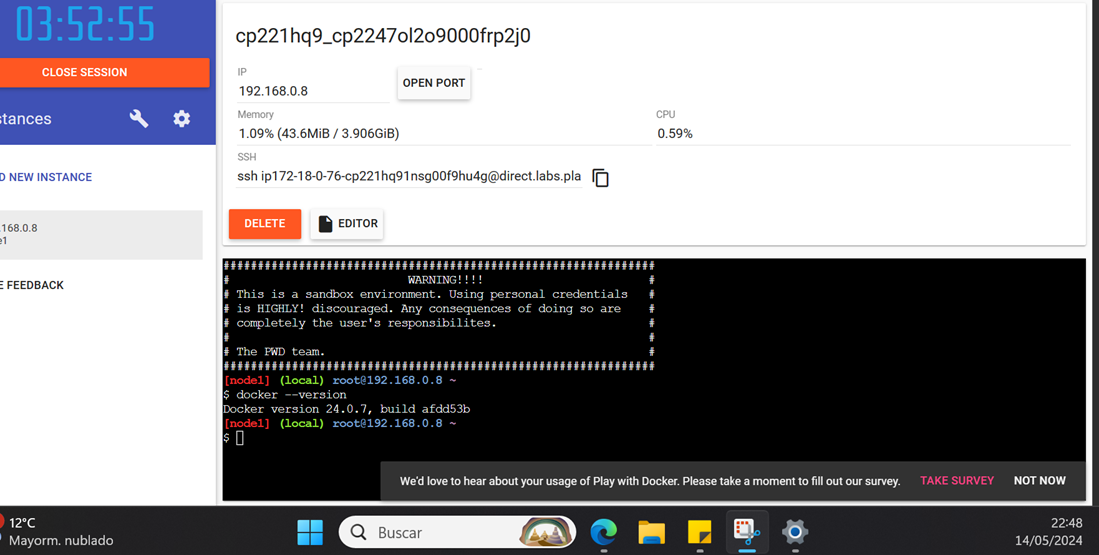
\includegraphics[width=0.75\linewidth]{docker3.png} % This is setting the figure to be .75x the width of the line. This can go all the way from 0.1 to 1 (and beyond, but then you're outside the page).
    \label{fig:OverallEffect}
\end{figure}

Podemos observar que la instancia levantada en play with docker nos proporciona una ip la que es útil a la hora de inicializar contenedores con los puertos utilicemos. 
Para probar el uso de docker y sus ventajas vamos a desplegar en nuestra instancia la página de JUICE-SHOP. 

Para acceder a JUICE-SHOP nos dirigimos al hub de docker oficial para poder descargar la imagen

\begin{figure}[H]
    \centering
    \caption{Dockerhub Juice-Shop.}
    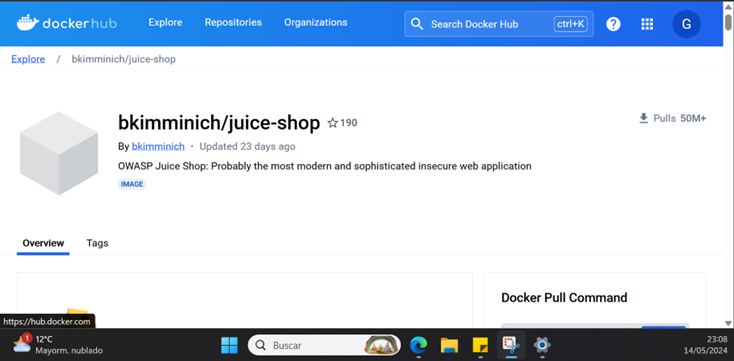
\includegraphics[width=0.75\linewidth]{docker4.png} % This is setting the figure to be .75x the width of the line. This can go all the way from 0.1 to 1 (and beyond, but then you're outside the page).
    \label{fig:OverallEffect}
\end{figure}

Dentro de nuestra instancia utilizamos los comandos:

\begin{enumerate}
  \item docker pull bkimminich/juice-shop:latest
  \item  docker run --rm -p 3000:3000 bkimminich/juice-shop
\end{enumerate}

Una vez ejecutados los comandos se desplegará la página de JUICE-SHOP en el puerto 3000. Para poder visualizar la página, el entorno de play with docker es intuitivo ya que al detectar que levanto un contenedor que utiliza un puerto este nos despliega un icono con el puerto disponible.

\begin{figure}[H]
    \centering
    \caption{Consola play with Docker: contenedor activo.}
    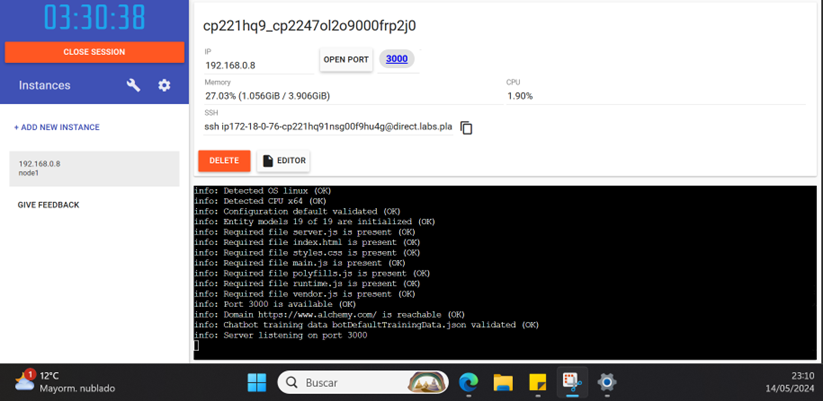
\includegraphics[width=0.75\linewidth]{docker5.png} % This is setting the figure to be .75x the width of the line. This can go all the way from 0.1 to 1 (and beyond, but then you're outside the page).
    \label{fig:OverallEffect}
\end{figure}

Al pinchar en el icono del puerto se abre una ventana con la página desplegada desde docker.

\begin{figure}[H]
    \centering
    \caption{Uso de comando nmap juice-shop.herokuapp.com.}
    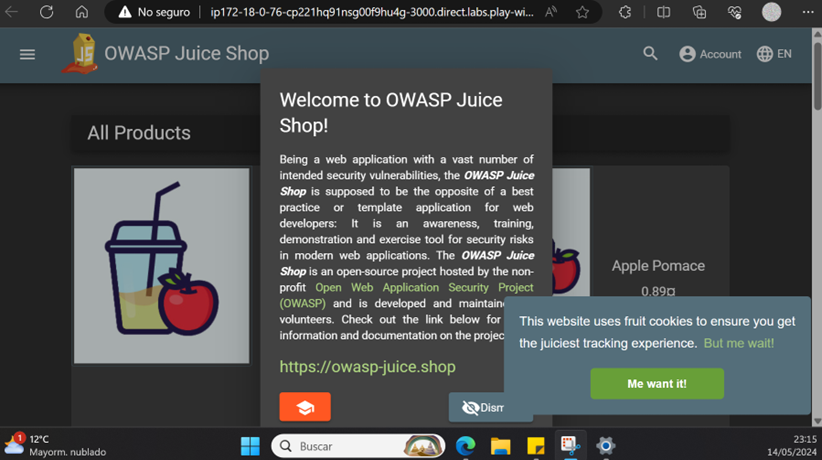
\includegraphics[width=0.75\linewidth]{docker6.png} % This is setting the figure to be .75x the width of the line. This can go all the way from 0.1 to 1 (and beyond, but then you're outside the page).
    \label{fig:OverallEffect}
\end{figure}

\section{\large Actividad 4}

\subsection{¿Qué es Phishing?} 
Proviene de la palabra en inglés fishing que significa pescar. El phishing es un tipo de ataque que comienza con un señuelo cuando recibes un correo electrónico que parece ser de una remitente confiable, tiene un alto sentido de urgencia y te solicita una acción inmediata como abrir un enlace a un sitio falso, descargar archivos o enviar información personal como usuarios y contraseñas. 
\noindent \maskCitet{phishing}\\

\subsection{¿Qué es phishingquiz?} 

Es una herramienta que ayuda a identificar maniobras de intentos de phishing donde el usuario ira pasando un total de 8 preguntas las que están basadas en casos lo más reales posibles para que el usuario se vaya concientizando en los detalles mínimos en los que podemos ser víctimas de robo de información u otro acontecimiento no esperado.

\subsection{Respondiendo phishingquiz} 

Para iniciar con la actividad ingresamos a la página Take Jigsaw’s phishing quiz. (s. f.-b). https://phishingquiz.withgoogle.com/  \noindent \maskCitet{phishingQuiz}\\  Luego seleccionamos el botón HACER EL TEST y se nos desplegara un pop up donde debemos ingresar nombre (real o ficticio) y correo electrónico. Luego hacemos clic en el botón EMPEZAR.

\begin{figure}[H]
    \centering
    \caption{Test phishingquiz.}
    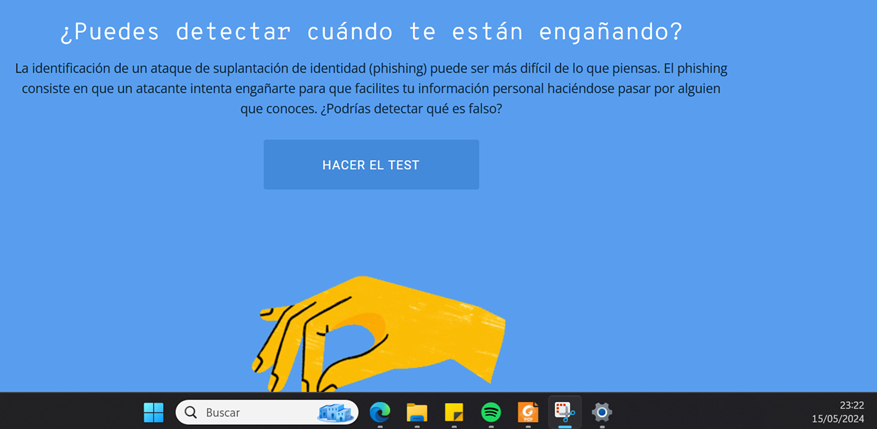
\includegraphics[width=0.75\linewidth]{phishing1.png} % This is setting the figure to be .75x the width of the line. This can go all the way from 0.1 to 1 (and beyond, but then you're outside the page).
    \label{fig:OverallEffect}
\end{figure}

Se nos abrirá la primera pregunta de un total de 8, donde se nos consultar si la muestra es Phishing o legitimo.

\begin{figure}[H]
    \centering
    \caption{Primera pregunta phishingquiz.}
    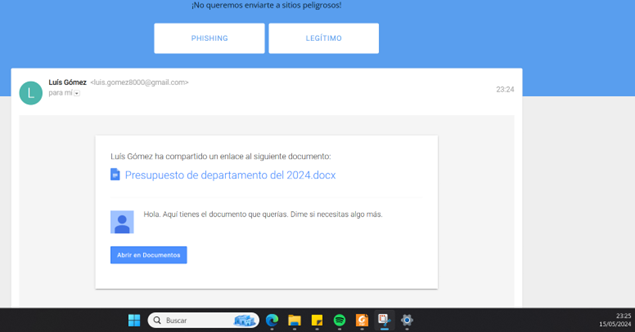
\includegraphics[width=0.75\linewidth]{phishing2.png} % This is setting the figure to be .75x the width of the line. This can go all the way from 0.1 to 1 (and beyond, but then you're outside the page).
    \label{fig:OverallEffect}
\end{figure}

Al analizar el primer test podemos considerar que es un correo de phishing debido a que el archivo adjunto supuestamente está en Google drive, pero no cumple con lo principal que es tener https (TLS activo), también el DNS del enlace no es un DNS valido de drive ya que el dns que se ocupa es https://drive.google.com/drive/

\begin{figure}[H]
    \centering
    \caption{Primera pregunta phishingquiz URL engañoza.}
    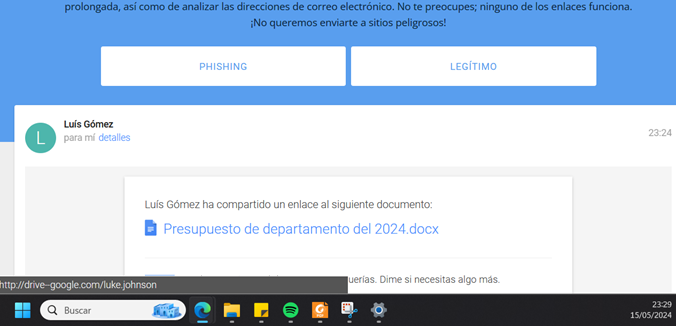
\includegraphics[width=0.75\linewidth]{phishing3.png} % This is setting the figure to be .75x the width of the line. This can go all the way from 0.1 to 1 (and beyond, but then you're outside the page).
    \label{fig:OverallEffect}
\end{figure}

Al seleccionar que es phishing la aplicación nos da por correcta la alternativa.

\begin{figure}[H]
    \centering
    \caption{Primera pregunta phishingquiz respuesta.}
    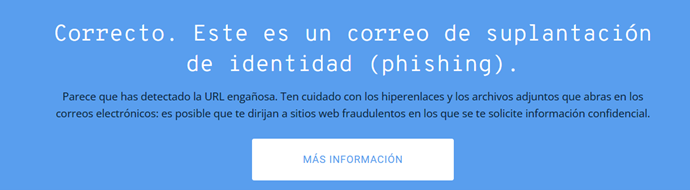
\includegraphics[width=0.75\linewidth]{phishing4.png} % This is setting the figure to be .75x the width of the line. This can go all the way from 0.1 to 1 (and beyond, but then you're outside the page).
    \label{fig:OverallEffect}
\end{figure}

El segundo caso nos expone en el contexto de recibir un correo con noreply (emails que normalmente son utilizados para no respuesta) Para este caso al igual que el primero tampoco confiaría del correo debido a que el enlace adjunto también apunta a un enlace no seguro http. También nos podemos percatar que el remitente del email lleva por nombre efacks que no es igual que el eFax.

\begin{figure}[H]
    \centering
    \caption{Segunda pregunta phishingquiz URL engañoza.}
    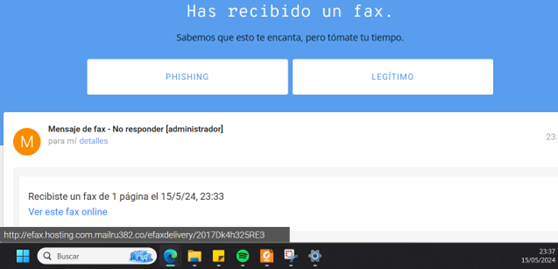
\includegraphics[width=0.75\linewidth]{phishing5.png} % This is setting the figure to be .75x the width of the line. This can go all the way from 0.1 to 1 (and beyond, but then you're outside the page).
    \label{fig:OverallEffect}
\end{figure}

El tercer caso nos coloca el envío de un email de parte de alguien con un correo electrónico poco común ya que solo nos indica un mensaje muy corto además al colocar el puntero sobre el enlace este nos apunta a una dirección que no es la de Google drive.

\begin{figure}[H]
    \centering
    \caption{Tercer pregunta phishingquiz.}
    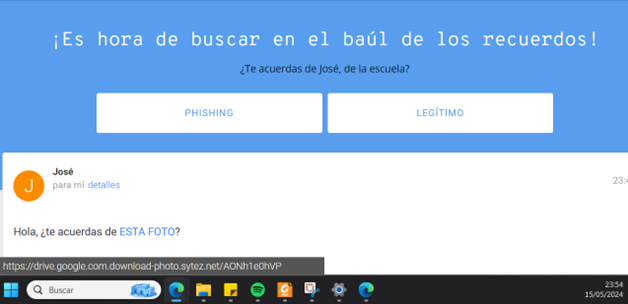
\includegraphics[width=0.75\linewidth]{phishing6.png} % This is setting the figure to be .75x the width of the line. This can go all the way from 0.1 to 1 (and beyond, but then you're outside the page).
    \label{fig:OverallEffect}
\end{figure}

En el cuarto caso se expone un correo de no-reply de parte de la empresa de almacenamiento de datos dropbox. Para alguien que esté utilizando Dropbox y haya llenado su almacenamiento es común que llegue este tipo de correos, lo poco común es el nombre del emisor de correo ya que es compuesto a nombre de dropbox pero no tiene un nombre con caracteres extraños. También podemos observar que al poner el cursor sobre los enlaces estos muestran páginas con el DNS principal de dropbox. Por lo cual este email se ve confiable a primera impresión.

\begin{figure}[H]
    \centering
    \caption{Cuarta pregunta phishingquiz.}
    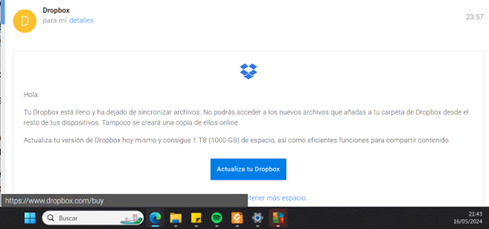
\includegraphics[width=0.75\linewidth]{phishing7.png} % This is setting the figure to be .75x the width of the line. This can go all the way from 0.1 to 1 (and beyond, but then you're outside the page).
    \label{fig:OverallEffect}
\end{figure}

El quinto caso es un mail común de envío de documento formato PDF. Podemos verificar que están relacionados los nombres del emisor con respecto a su correo electrónico.  Pero si leemos detenidamente lo que nos dice el texto bajo el Titulo este nos indica el mail remitente es muy parecido, pero no igual al que estamos acostumbrados a recibir. Por tanto, confirmamos que este correo no es legítimo y es tipo suplantación de identidad.

\begin{figure}[H]
    \centering
    \caption{Quinta pregunta phishingquiz.}
    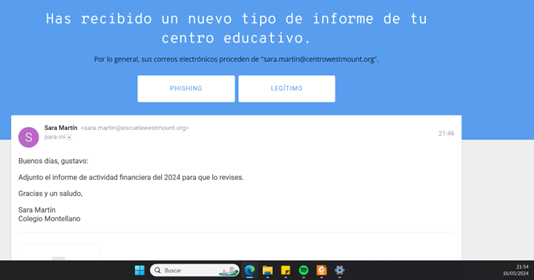
\includegraphics[width=0.75\linewidth]{phishing8.png} % This is setting the figure to be .75x the width of the line. This can go all the way from 0.1 to 1 (and beyond, but then you're outside the page).
    \label{fig:OverallEffect}
\end{figure}

El sexto quiz trata sobre los correos que recibimos normalmente cuando accedemos a nuestras cuentas de mail. Por lo general los correos de acceso de Gmail no indican que alguien tiene tu contraseña solo alertan de un inicio de sesión en un equipo con un sistema operativo y proporcionan un botón de enlace para verificar el historial de alertas de acceso de los últimos 28 días. También podemos verificar que el colocar el puntero sobre el botón este nos redirige a un enlace que no es enlace oficial de cuentas de Google https://myaccount.google.com/notifications  y ademas es un sitio sin TLS.

\begin{figure}[H]
    \centering
    \caption{Sexta pregunta phishingquiz.}
    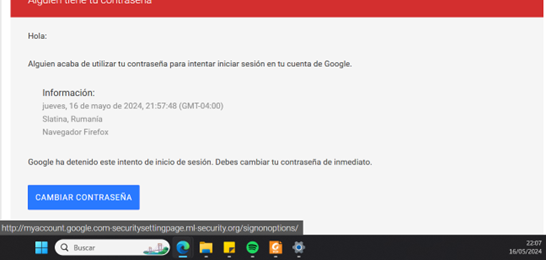
\includegraphics[width=0.75\linewidth]{phishing9.png} % This is setting the figure to be .75x the width of the line. This can go all the way from 0.1 to 1 (and beyond, but then you're outside the page).
    \label{fig:OverallEffect}
\end{figure}

El séptimo quiz nos informa sobre el ataque de mi cuenta de email. Los criterios para tomar en cuenta en este análisis están por parte del remitente ya que proviene de una cuenta de google.support  y no de una cuenta de Google terminada en .com también el enlace de cambiar contraseña redirige a un enlace no valido de Google.

\begin{figure}[H]
    \centering
    \caption{Septima pregunta phishingquiz.}
    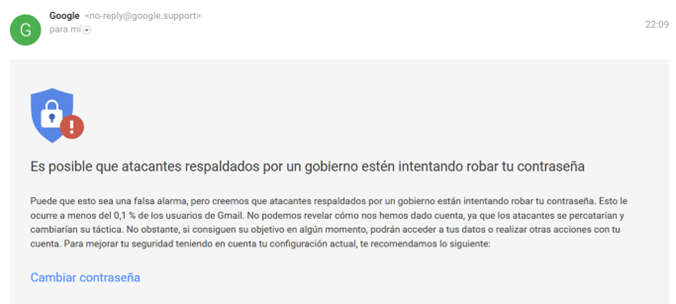
\includegraphics[width=0.75\linewidth]{phishing10.png} % This is setting the figure to be .75x the width of the line. This can go all the way from 0.1 to 1 (and beyond, but then you're outside the page).
    \label{fig:OverallEffect}
\end{figure}

Lo normal de las cuentas de información de Google son por el remitente no-reply@accounts.google.com que son remitentes validos de parte de Google.

El último quiz trata de cuando nos registramos en alguna página y se nos solicita autorización de acceder a cierta información de mi correo electrónico. Para este caso podemos analizar que el nombre del remitente Triplt coincide con el DNS pero, aunque en un principio resulto ser engorroso ya que el remitente se anuncia con título TripIt y no Tripit y eso en primera vista puede dar una leve sospecha.

\begin{figure}[H]
    \centering
    \caption{Octava pregunta phishingquiz.}
    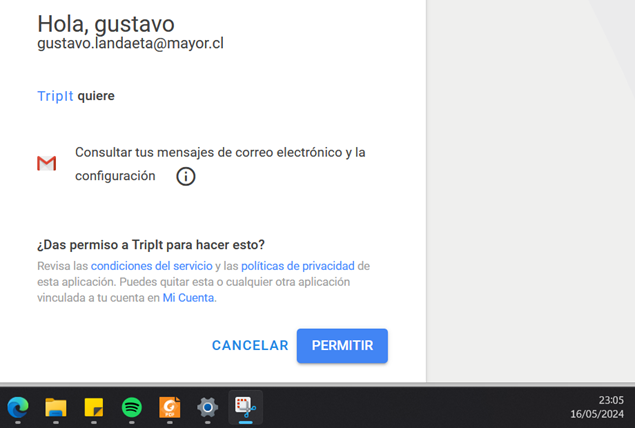
\includegraphics[width=0.75\linewidth]{phishing11.png} % This is setting the figure to be .75x the width of the line. This can go all the way from 0.1 to 1 (and beyond, but then you're outside the page).
    \label{fig:OverallEffect}
\end{figure}

Pero si analizamos en profundidad los enlaces a los cuales redirecciona podemos verificar que es un enlace valido https://www.tripit.com.

\newpage

\section{\large Actividad 5}

\subsection{¿Qué es OSINT Framework?}

OSINT Framework es una plataforma que, según las categorías que define, sugiere diferentes herramientas para realizar búsquedas y análisis que apoyen investigaciones de inteligencia en fuentes abiertas, desde una perspectiva no intrusiva.

\subsection{¿Qué uso se le puede dar a OSINT Framework?}

Dentro de los múltiples usos que se le pueden dar a OSINT Framework está la investigación de ciberseguridad (identificar patrones y correlaciones entre distintos incidentes de seguridad, rastrear cibercriminales), análisis de seguridad (identificar vulnerabilidades y amenazas a partir de información pública), recopilación de información (búsqueda de datos específicos de organizaciones, personas, geolocalización) y periodismo de investigación (descubrir y verificar información para sus artículos).

\subsection{¿En qué fase el hacking ético se pudiese usar el OSINT Framework?}

¿En qué fase el hacking ético se pudiese usar el OSINT Framework?
Es en la fase de Reconocimiento donde principalmente se puede usar, ya que es la primera etapa del proceso, en donde el propósito es la recopilación de información sobre el objetivo sin interactuar directamente con él, esto puede contemplar: la identificación de nombres de dominio, direcciones IP, empleados, directivos, tecnologías y sistemas operativos en uso, entre otros.

El acceso a OSINT Framework es a través de la siguiente web: https://osintframework.com/

\begin{figure}[H]
\centering
\caption{Vista Inicial de OSINT Framework.}
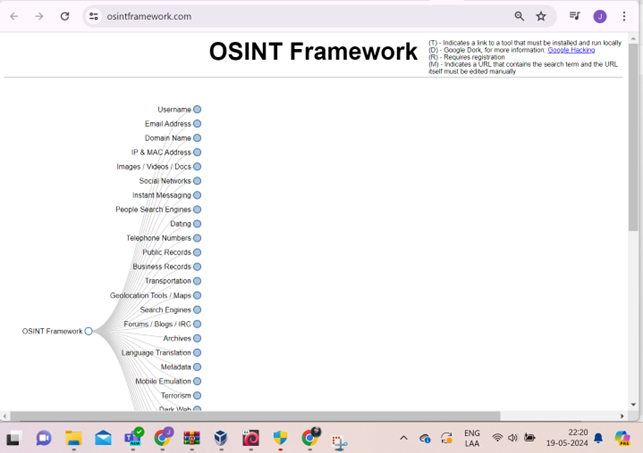
\includegraphics[width=0.75\linewidth]{osi1.png} % This is setting the figure to be .75x the width of the line. This can go all the way from 0.1 to 1 (and beyond, but then you're outside the page).
\label{fig:OverallEffect}
\end{figure}

La plataforma, para algunas herramientas establece 4 indicadores, los cuales describe en la parte superior derecha del sitio. Estos nos ayudan a identificar si las herramientas se tratan de:

\begin{itemize}
\item[] - (T): Enlace de una herramienta para instalar y ejecutar en nuestro equipo.
\item[] - (D): Uso de Google Dork.
\item[] - (R): Herramienta que requiere de un registro en una plataforma, previo a su uso.
\item[] - (M): Aplicativo web, que en su URL se debe configurar o editar manualmente el término de búsqueda. 
\end{itemize}

\begin{figure}[H]
\centering
\caption{Leyenda de indicadores en OSINT Framework.}
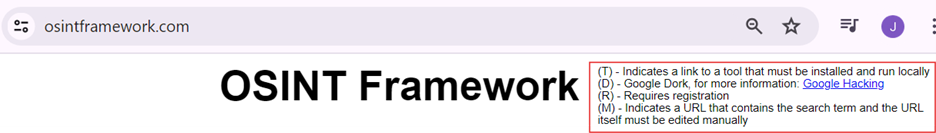
\includegraphics[width=0.75\linewidth]{osi2.png} % This is setting the figure to be .75x the width of the line. This can go all the way from 0.1 to 1 (and beyond, but then you're outside the page).
\label{fig:OverallEffect}
\end{figure}

\subsection{Social-Searcher}

La herramienta seleccionada fue “Social-Searcher”, su sitio web es https://www.social-searcher.com/. Esta herramienta permite rastrear lo que se dice de una marca, empresa, persona, producto o servicio, ello a través del monitoreo en tiempo real de menciones en redes sociales y sitios web. En OSINT Framework se ubica dentro de la categoría “Social Networks”, a su vez en la subcategoría “Search”.

\begin{figure}[H]
\centering
\caption{Ubicación de Social-Searcher en OSINT Framework.}
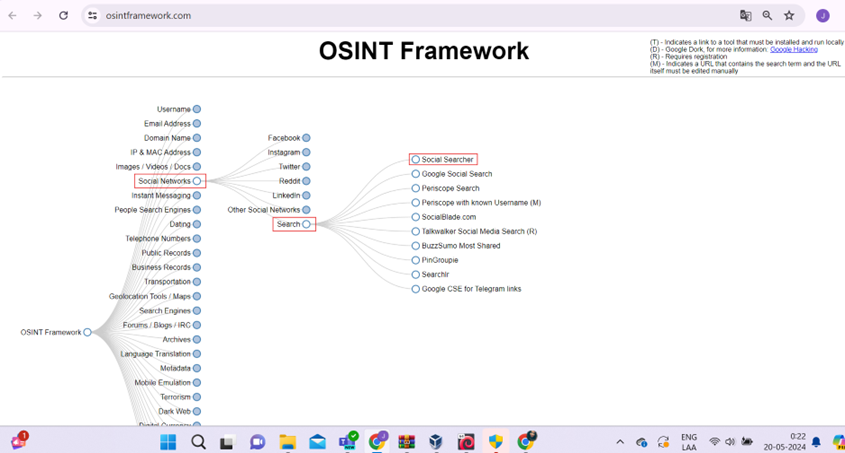
\includegraphics[width=0.75\linewidth]{osi3.png} % This is setting the figure to be .75x the width of the line. This can go all the way from 0.1 to 1 (and beyond, but then you're outside the page).
\label{fig:OverallEffect}
\end{figure}

Social-Searcher tiene una versión gratuita y otras pagas, ofreciendo funciones avanzadas para generar alertar por correo electrónico, exportación de datos y también expone un API para facilitar su integración con otras herramientas.

\begin{figure}[H]
\centering
\caption{Inicio de Social-Searcher.}
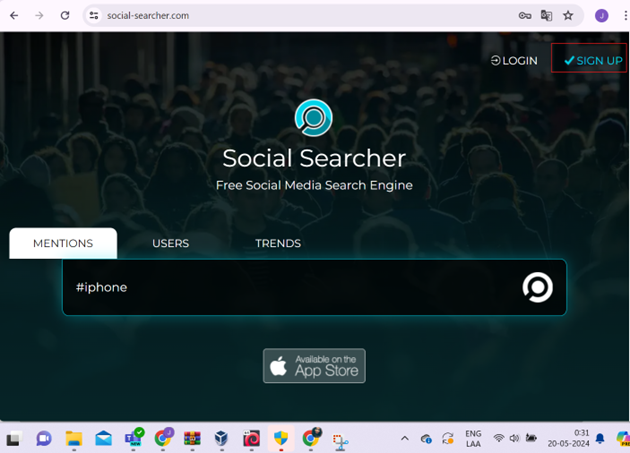
\includegraphics[width=0.75\linewidth]{osi4.png} % This is setting the figure to be .75x the width of the line. This can go all the way from 0.1 to 1 (and beyond, but then you're outside the page).
\label{fig:OverallEffect}
\end{figure}

\subsection{Utilidades de Social-Searcher en Ciberseguridad}

Esta herramienta facilita el monitore en tiempo real de menciones en la web y redes sociales, lo cual es de utilidad para:

\begin{itemize}
\item[] - Detectar Amenazas, por medio de la identificación de menciones sobre vulnerabilidades y/o ataques inminentes.
\item[] - Analizar Sentimientos Implícitos, evaluando el tono de mensajes, publicaciones o interacciones respecto a una marca, empresa, producto o persona, con el fin de detectar posibles riesgos reputacionales.
\item[] - Monitorear Influencers, con el seguimiento a personas o medios de comunicación influyentes que puedan impactar la seguridad y reputación de la empresa.
\item[] - Identificar Alertas en Tiempo Real, recibiendo notificaciones de forma instantánea sobre menciones específicas.
\end{itemize}

\subsection{Etapa de Reconocimiento de Hancking Ético y Social-Searcher}

La herramienta Social-Searcher puede aportar significativamente en la etapa de reconocimiento del Hacking Ético al ser una fuente de:

\begin{itemize}
\item[] - Recopilación de Información, entregando contenido sobre una organización o individuo derivada del monitoreo de menciones y actividades en redes sociales y/o la web.
\item[] - Detección de Exposiciones, encontrar datos sensibles que puedan haber sido publicados de forma accidentalmente o no accidental.
\item[] - Detección de Amenazas Internas o Externas, analizando los sentimientos impresos en las publicaciones de trabajadores, consumidores o público en general.
\item[] - Identificación de Actores Clave, reconociendo a personas que podrían representar una fuente de información relevante u objetivos de ataques de ingeniería social.
\end{itemize}

\subsection{Debilidades que Considerar Respecto al Uso de Social-Searcher}

Social-Searcher como herramienta tiene algunas limitaciones o propiedades desfavorables que considerar ante su uso, tales como:

\begin{itemize}
\item[] - Limitaciones funcionales en versión gratuita, en su mayoría las características avanzadas sólo están disponibles en las versiones pagas.
\item[] - Dependencia de fuentes públicas, lo que puede limitar la profundidad del análisis, así como la veracidad de la información.
\item[] - Ruido en los datos, lo que implica el tratamiento de una gran cantidad de datos irrelevantes, para hallar información crítica.
\item[] - Plantea preocupaciones respecto a la privacidad y ética en la recopilación de datos.
\end{itemize}

\subsection{Caso Filtración Banco Santander}

Para el desarrollo del ejercicio con la herramienta Social-Searcher se seleccionó la temática de “Filtración de Datos del Banco Santander”. 
En primer lugar, se debe acceder al sitio web de la herramienta (https://www.social-searcher.com), se debe registrar y luego validar la cuenta por medio de un correo electrónico que se enviará a la dirección registrada.

\begin{figure}[H]
\centering
\caption{Pantalla de inicio - Sección de Login.}
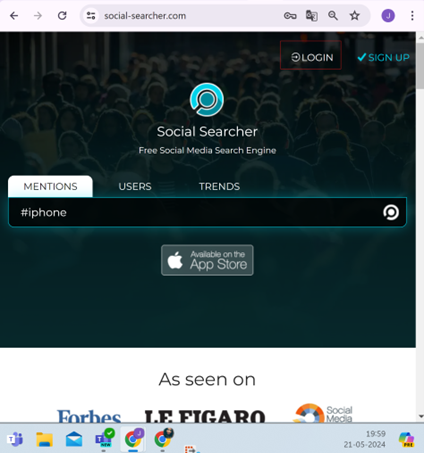
\includegraphics[width=0.75\linewidth]{osi5.png} % This is setting the figure to be .75x the width of the line. This can go all the way from 0.1 to 1 (and beyond, but then you're outside the page).
\label{fig:OverallEffect}
\end{figure}

\begin{figure}[H]
\centering
\caption{Pantalla de inicio - Sección de Login - Registro.}
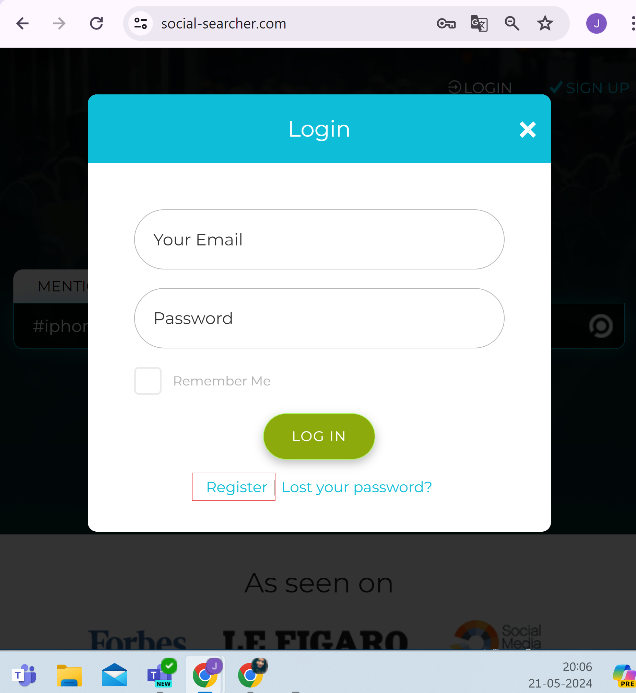
\includegraphics[width=0.75\linewidth]{osi6.png} % This is setting the figure to be .75x the width of the line. This can go all the way from 0.1 to 1 (and beyond, but then you're outside the page).
\label{fig:OverallEffect}
\end{figure}

\begin{figure}[H]
\centering
\caption{Pantalla de registro en Social-Searcher.}
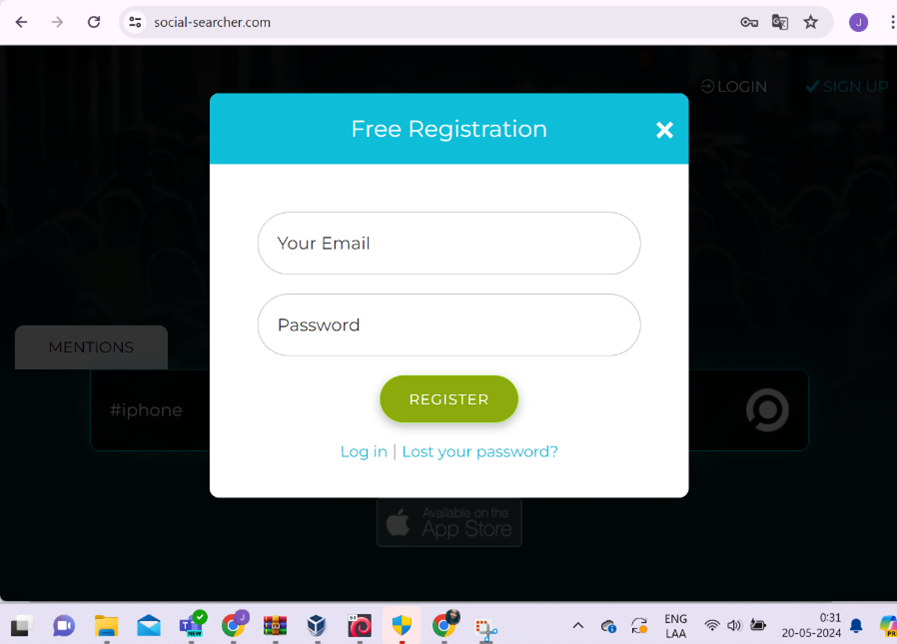
\includegraphics[width=0.75\linewidth]{osi7.png} % This is setting the figure to be .75x the width of the line. This can go all the way from 0.1 to 1 (and beyond, but then you're outside the page).
\label{fig:OverallEffect}
\end{figure}

Luego, se inicia la búsqueda del objetivo, lo que se puede realizar por frases mencionadas, usuarios o tema en tendencia, la primera de estas fue la empleada en la presente actividad.

\begin{figure}[H]
\centering
\caption{Búsqueda por mención. }
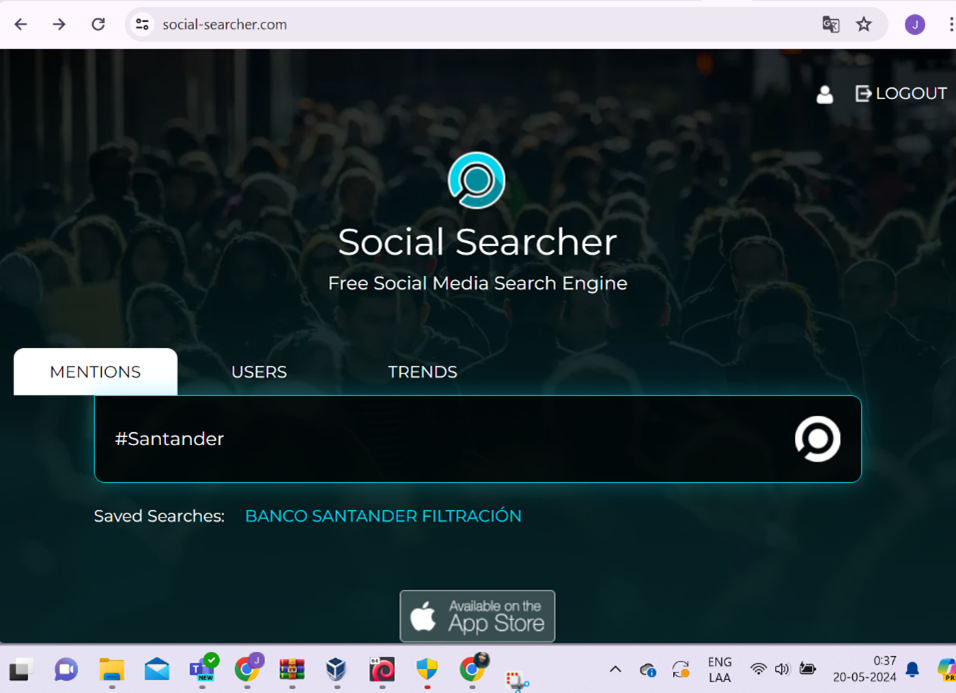
\includegraphics[width=0.75\linewidth]{osi8.png} % This is setting the figure to be .75x the width of the line. This can go all the way from 0.1 to 1 (and beyond, but then you're outside the page).
\label{fig:OverallEffect}
\end{figure}

Según la búsqueda básica, se obtienen los primeros resultados, en total la herramienta identificó 479 menciones relacionadas con el objetivo de 207 usuarios.

\begin{figure}[H]
\centering
\caption{Panel de resultado general. }
\includegraphics[width=0.75\linewidth]{osi9.png} % This is setting the figure to be .75x the width of the line. This can go all the way from 0.1 to 1 (and beyond, but then you're outside the page).
\label{fig:OverallEffect}
\end{figure}

Para una búsqueda más efectiva, la herramienta permite la configuración de parámetros como palabras claves, fuentes, tipo (foto, video, enlace, entre otros), idioma, fecha y sentimientos sobre la información.

\begin{figure}[H]
\centering
\caption{Configuración por palabras. }
\includegraphics[width=0.75\linewidth]{osi10.png} % This is setting the figure to be .75x the width of the line. This can go all the way from 0.1 to 1 (and beyond, but then you're outside the page).
\label{fig:OverallEffect}
\end{figure}

\begin{figure}[H]
\centering
\caption{Configuración por fuentes. }
\includegraphics[width=0.75\linewidth]{osi11.png} % This is setting the figure to be .75x the width of the line. This can go all the way from 0.1 to 1 (and beyond, but then you're outside the page).
\label{fig:OverallEffect}
\end{figure}

\begin{figure}[H]
\centering
\caption{Configuración por tipo de información e idioma.}
\includegraphics[width=0.75\linewidth]{osi12.png} % This is setting the figure to be .75x the width of the line. This can go all the way from 0.1 to 1 (and beyond, but then you're outside the page).
\label{fig:OverallEffect}
\end{figure}

Luego de aplicar las configuraciones correspondientes y ajustadas a las necesidades de la investigación, se obtiene un resultado refinado, ahora de 62 menciones de 26 usuarios. 

La herramienta también nos permite ordenar los resultados por fecha o popularidad de la información. 

\begin{figure}[H]
\centering
\caption{Nuevos resultados con configuraciones aplicadas.}
\includegraphics[width=0.75\linewidth]{osi13.png} % This is setting the figure to be .75x the width of the line. This can go all the way from 0.1 to 1 (and beyond, but then you're outside the page).
\label{fig:OverallEffect}
\end{figure}

\begin{figure}[H]
\centering
\caption{Funcionalidad disponible para ordenar la información.}
\includegraphics[width=0.75\linewidth]{osi14.png} % This is setting the figure to be .75x the width of the line. This can go all the way from 0.1 to 1 (and beyond, but then you're outside the page).
\label{fig:OverallEffect}
\end{figure}

La herramienta permite exportar la información obtenida de la búsqueda en formato .csv.

\begin{figure}[H]
\centering
\caption{Exportar resultados.}
\includegraphics[width=0.75\linewidth]{osi15.png} % This is setting the figure to be .75x the width of the line. This can go all the way from 0.1 to 1 (and beyond, but then you're outside the page).
\label{fig:OverallEffect}
\end{figure}

\begin{figure}[H]
\centering
\caption{Extracto de resultado exportado.}
\includegraphics[width=0.75\linewidth]{osi16.png} % This is setting the figure to be .75x the width of the line. This can go all the way from 0.1 to 1 (and beyond, but then you're outside the page).
\label{fig:OverallEffect}
\end{figure}

La herramienta realiza analítica de la información y presenta estadísticas detalladas según las categorías general (cronología de publicaciones, fuentes de información, día y hora de las publicaciones, y hashtag incluidos en las publicaciones), sentimiento (positivo, negativo y neutro por fuente de información), usuarios (activos y populares por fuente de información), enlaces (por dominio e identificación de enlaces populares), tipos de contenido (video, foto y enlace, medidos por fuente de información y popularidad de la publicación) y palabras clave (1, 2 o 3 palabras clave).

\begin{figure}[H]
\centering
\caption{Estadística y analítica general - Cronología.}
\includegraphics[width=0.75\linewidth]{osi17.png} % This is setting the figure to be .75x the width of the line. This can go all the way from 0.1 to 1 (and beyond, but then you're outside the page).
\label{fig:OverallEffect}
\end{figure}

\begin{figure}[H]
\centering
\caption{Estadística y analítica general - Fuente de Información.}
\includegraphics[width=0.75\linewidth]{osi18.png} % This is setting the figure to be .75x the width of the line. This can go all the way from 0.1 to 1 (and beyond, but then you're outside the page).
\label{fig:OverallEffect}
\end{figure}

\begin{figure}[H]
\centering
\caption{Estadística y analítica general – Publicaciones por día y hora.}
\includegraphics[width=0.75\linewidth]{osi19.png} % This is setting the figure to be .75x the width of the line. This can go all the way from 0.1 to 1 (and beyond, but then you're outside the page).
\label{fig:OverallEffect}
\end{figure}

\begin{figure}[H]
\centering
\caption{Estadística y analítica general - Hashtags.}
\includegraphics[width=0.75\linewidth]{osi20.png} % This is setting the figure to be .75x the width of the line. This can go all the way from 0.1 to 1 (and beyond, but then you're outside the page).
\label{fig:OverallEffect}
\end{figure}

\begin{figure}[H]
\centering
\caption{Estadística y analítica por sentimiento.}
\includegraphics[width=0.75\linewidth]{osi21.png} % This is setting the figure to be .75x the width of the line. This can go all the way from 0.1 to 1 (and beyond, but then you're outside the page).
\label{fig:OverallEffect}
\end{figure}

\begin{figure}[H]
\centering
\caption{Estadística y analítica por usuario.}
\includegraphics[width=0.75\linewidth]{osi22.png} % This is setting the figure to be .75x the width of the line. This can go all the way from 0.1 to 1 (and beyond, but then you're outside the page).
\label{fig:OverallEffect}
\end{figure}

\begin{figure}[H]
\centering
\caption{Estadística y analítica por usuarios – Usuarios populares y activos.}
\includegraphics[width=0.75\linewidth]{osi23.png} % This is setting the figure to be .75x the width of the line. This can go all the way from 0.1 to 1 (and beyond, but then you're outside the page).
\label{fig:OverallEffect}
\end{figure}

\begin{figure}[H]
\centering
\caption{Estadística y analítica por enlaces.}
\includegraphics[width=0.75\linewidth]{osi24.png} % This is setting the figure to be .75x the width of the line. This can go all the way from 0.1 to 1 (and beyond, but then you're outside the page).
\label{fig:OverallEffect}
\end{figure}

\begin{figure}[H]
\centering
\caption{Estadística y analítica por enlaces – Enlaces populares.}
\includegraphics[width=0.75\linewidth]{osi25.png} % This is setting the figure to be .75x the width of the line. This can go all the way from 0.1 to 1 (and beyond, but then you're outside the page).
\label{fig:OverallEffect}
\end{figure}

\begin{figure}[H]
\centering
\caption{Estadística y analítica por tipo de contenido.}
\includegraphics[width=0.75\linewidth]{osi26.png} % This is setting the figure to be .75x the width of the line. This can go all the way from 0.1 to 1 (and beyond, but then you're outside the page).
\label{fig:OverallEffect}
\end{figure}

\begin{figure}[H]
\centering
\caption{Estadística y analítica por palabras clave.}
\includegraphics[width=0.75\linewidth]{osi27.png} % This is setting the figure to be .75x the width of the line. This can go all the way from 0.1 to 1 (and beyond, but then you're outside the page).
\label{fig:OverallEffect}
\end{figure}

\newpage

\section{\large Actividad 6}

\subsection{¿Qué es un motor de búsqueda?} 

Son plataformas que se encuentran escaneando activamente los diferentes servidores y IPs que se encuentran con acceso a internet, estos escaneos recolección información de ubicación de los hosts, puertos, versione, entre otros datos relevantes para conocer sobre un target que se desee recolectar información de forma pasiva.

\subsection{Caso de estudio: Payku} 

Payku es una plataforma de pagos, para pequeñas y medianas empresas con el fin de facilitar y agilizar las transacciones entre sus clientes. Para este caso se analizará la url app.payku.cl utilizando los tres motores de búsquedas mas conocidos: Shodan, Censys y Zoomeye.

\subsection{Recolección pasiva de información a través de motores de búsqueda}

\subsubsection{Shodan}

Se debe ingresar a la URL https://www.shodan.io/ y en el buscador colocamos app.payku.cl.

\begin{figure}[H]
    \centering
    \caption{Motor Shodan}
    \includegraphics[width=0.75\linewidth]{ac61.png} % This is setting the figure to be .75x the width of the line. This can go all the way from 0.1 to 1 (and beyond, but then you're outside the page).
    \label{fig:OverallEffect}
\end{figure}

En la Figura 47 (cambiar) se puede observar que el motor no tiene ninguna información de esta URL, esto puede ser porque el representante de Payku solicito que se bajara la información de Shodan.

\begin{figure}[H]
    \centering
    \caption{Resultados del motor Shodan}
    \includegraphics[width=0.75\linewidth]{ac62.png} % This is setting the figure to be .75x the width of the line. This can go all the way from 0.1 to 1 (and beyond, but then you're outside the page).
    \label{fig:OverallEffect}
\end{figure}

\subsubsection{Zoomeye}

Se debe ingresar a la URL https://www.zoomeye.hk/ y en el buscador colocamos app.payku.cl.

\begin{figure}[H]
    \centering
    \caption{Motor Zoomeye}
    \includegraphics[width=0.75\linewidth]{ac63.png} % This is setting the figure to be .75x the width of the line. This can go all the way from 0.1 to 1 (and beyond, but then you're outside the page).
    \label{fig:OverallEffect}
\end{figure}

El motor Zoomeye consigue el resultado mostrado en la Figura 48 (cambiar).

\begin{figure}[H]
    \centering
    \caption{Resultado del motor Zoomeye}
    \includegraphics[width=0.75\linewidth]{ac64.png} % This is setting the figure to be .75x the width of the line. This can go all the way from 0.1 to 1 (and beyond, but then you're outside the page).
    \label{fig:OverallEffect}
\end{figure}

Teniendo un resultado, Zoomeye no tiene información relevantes de puertos ni servicios.

\begin{figure}[H]
    \centering
    \caption{Detalles de app.payku.cl del motos Zoomeye}
    \includegraphics[width=0.75\linewidth]{ac65.png} % This is setting the figure to be .75x the width of the line. This can go all the way from 0.1 to 1 (and beyond, but then you're outside the page).
    \label{fig:OverallEffect}
\end{figure}

\subsubsection{Censys}

Se debe ingresar a la URL https://search.censys.io/ y en el buscador colocamos app.payku.cl.

\begin{figure}[H]
    \centering
    \caption{Motor Censys}
    \includegraphics[width=0.75\linewidth]{ac66.png} % This is setting the figure to be .75x the width of the line. This can go all the way from 0.1 to 1 (and beyond, but then you're outside the page).
    \label{fig:OverallEffect}
\end{figure}

El motor Censys consigue el resultado mostrado en la Figura 48 (cambiar).

\begin{figure}[H]
    \centering
    \caption{Resultado del motor Censys}
    \includegraphics[width=0.75\linewidth]{ac67.png} % This is setting the figure to be .75x the width of the line. This can go all the way from 0.1 to 1 (and beyond, but then you're outside the page).
    \label{fig:OverallEffect}
\end{figure}

Censys mostro resultados mas favorables que los motores anteriores, dandonos información de los diferentes hosts, sistemas operativos, puertos, entre otras informaciones. En la Tabla 2 se centralizan los hallazgos de Censys para la busqueda de app.payku.cl.


\begin{table}[H]
    \caption{Información obtenida por el motor Censys.}
    \centering
   \resizebox{\textwidth}{!}{ \begin{tabular}{ccccc} %The c's here indicate the columns will be centered
        \hline 
         IP & Ubicación & Nube & Sistema Operativo & Puertos/Servicios\\
         \hline
         2800:6c0:3:0:0:0:0:1747 & Santa Fe, Argentina & Dattatec.com  & N/A & 21/FTP,80/HTTP,443/HTTP\\
          66.97.32.63 & Buenos Aires F.D., Argentina & Dattatec.com  & Linux & 21/FTP,80/HTTP,443/HTTP,3003/HTTP,3040/HTTP,3069/HTTP,5421/SSH,27017/MONGODB\\
	35.238.240.220 & Iowa, United States & GOOGLE-CLOUD-PLATFORM  & Linux & 22/SSH,80/HTTP\\
	34.72.183.120 & Iowa, United States & GOOGLE-CLOUD-PLATFORM  & Centos Linux & 443/HTTP\\
	34.27.136.109 & Iowa, United States & GOOGLE-CLOUD-PLATFORM  & Centos Linux & 443/HTTP\\
	34.132.125.83 & Iowa, United States & GOOGLE-CLOUD-PLATFORM  & Centos Linux & 443/HTTP\\
	35.188.197.195 & Iowa, United States & GOOGLE-CLOUD-PLATFORM  & Centos Linux & 443/HTTP\\
	35.239.233.140 & Iowa, United States & GOOGLE-CLOUD-PLATFORM  & Centos Linux & 443/HTTP\\
	35.232.54.194 & Iowa, United States & GOOGLE-CLOUD-PLATFORM  & Centos Linux & 443/HTTP\\
         \hline
    \end{tabular}}
    \label{tab:table_words}
\end{table}


\newpage

\section{\large Actividad 7}
%\noindent \maskCitet{cervantes1999}\\

\subsection{¿Qué es Nmap?} 
Es una herramienta de código abierto que permite escanear redes y sus puertos con el fin de identificar hosts, servicios en la red, vulnerabilidades y funcionalidades.

\subsection{Caso juice-shop.herokuapp.com} 
Para esta actividad se utilizo como target juice-shop.herokuapp.com, esta pagina se encuentra en el host de Heroku y la aplicación a analizar fue desarrollada por OWASP con el fin de practicar y utilizar diferentes herramientas para la búsqueda de vulnerabilidades.


En este caso se empezará con la búsqueda de puertos activos debido a que el scope de la recolección de información es directamente juice-shop.herokuapp.com, en caso de que se desee conocer que IP´s se encuentran en una red se podría utilizar el siguiente comando:
\newline

\begin{lstlisting}
nmap 192.168.1.1-254
\end{lstlisting}

La metodología que se debe utilizar para minimizar el tiempo de las pruebas y generar menos ruido es la siguiente: escanear la red para conocer las IP´s activas de la red, posteriormente los puertos de las IP´s halladas y por ultimo los servicios que corren en los puertos hallados, además de esto se pueden correr diferentes scripts que nos permiten conocer las posibles vulnerabilidades que se pueden conseguir en estos servicios.


\subsection{Búsqueda de puertos activos} 
Debido a que el target es una pagina web el siguiente comando nmap juice-shop.herokuapp.com, nos permitirá conocer su IP y los puertos que se encuentren activos, lo que nos permitirá tener una idea de cuales servicios pueden ser los que se encuentren activos.

\begin{table}[H]
    \caption{Información de puertos obtenidos con Nmap.}
    \centering
    \begin{tabular}{ccc} %The c's here indicate the columns will be centered
        \hline 
         Puerto & Estado & Servicio\\
         \hline
         80/tcp & Abierto & http\\
          443/tcp & Abierto & https\\
	8010/tcp & Abierto & xmpp\\
         \hline
    \end{tabular}
    \label{tab:table_words}
\end{table}

\begin{figure}[H]
    \centering
    \caption{Uso de comando nmap juice-shop.herokuapp.com.}
    \includegraphics[width=0.75\linewidth]{Imagen1.png} % This is setting the figure to be .75x the width of the line. This can go all the way from 0.1 to 1 (and beyond, but then you're outside the page).
    \label{fig:OverallEffect}
\end{figure}


\subsection{Búsqueda de versiones de servicios} 
Al tener definido los puertos que se encuentran abiertos, podremos conocer las versiones de estos servicios sin tener que escanear de nuevo todos los puertos asociados a juice-shop.herokuapp.com lo que disminuye el tiempo que toma a Nmap en el escaneo. El comando por utilizar será el siguiente:
\newline

\begin{lstlisting}
nmap -sV -p80,443,8010 juice-shop.herokuapp.com
\end{lstlisting}

\begin{itemize}
  \item[] - sV: Corresponde a la opción de búsqueda de versiones.
  \item[] - p: Puertos a escanear (si se desean escanear los mil más comunes usar -p-).
\end{itemize}


\begin{table}[H]
    \caption{Información de versiones obtenidos con Nmap.}
    \centering
    \begin{tabular}{cccc} %The c's here indicate the columns will be centered
        \hline 
         Puerto & Estado & Servicio & Version\\
         \hline
         80/tcp & Abierto & http & Heroku\\
          443/tcp & Abierto & ssl/https & Heroku\\
	8010/tcp & Abierto & ssl/xmpp & N/A\\
         \hline
    \end{tabular}
    \label{tab:table_words}
\end{table}

\begin{figure}[H]
    \centering
    \caption{Uso de comando nmap -sV -p80,443,8010 juice-shop.herokuapp.com}
    \includegraphics[width=0.75\linewidth]{Imagen2.png} % This is setting the figure to be .75x the width of the line. This can go all the way from 0.1 to 1 (and beyond, but then you're outside the page).
    \label{fig:OverallEffect}
\end{figure}

\subsection{Búsqueda de vulnerabilidades en servicios utilizando Scripts de Nmap} 
Otra importante cualidad de esta herramienta es la posibilidad de correr script desarrollados en Lua que nos permiten detectar vulnerabilidades en los servicios, además de permitirnos generar nuestros propios scripts y aplicarlos a través de Nmap. Para utilizar los scripts base de Nmap se utiliza el siguiente comando:
\newline

\begin{lstlisting}
nmap -sC -p80,443,8010 juice-shop.herokuapp.com
\end{lstlisting}

\begin{itemize}
  \item[] - sC: Corresponde a la opción de scripts Nmap.
  \item[] - p: Puertos a escanear (si se desean escanear los mil más comunes usar -p-).
\end{itemize}

\begin{figure}[H]
    \centering
    \caption{Uso de comando nmap -sC -p80,443,8010 juice-shop.herokuapp.com}
    \includegraphics[width=0.75\linewidth]{Imagen3.png} % This is setting the figure to be .75x the width of the line. This can go all the way from 0.1 to 1 (and beyond, but then you're outside the page).
    \label{fig:OverallEffect}
\end{figure}

De esto podemos observar lo siguiente:

\begin{enumerate}
  \item Para los puertos 80 y 8010 se encuentran habilitados verbos http HEAD, GET, PUT, DELETE y PATCH.
  \item En el puerto 80 se puede observar que se tiene un directorio ftp.
  \item En los puertos 80 y 8010 se puede observar que tiene un archivo robots.txt.
\end{enumerate}

Para obtener mas información de este target se deberán utilizar otros scripts mas especializados o otras herramientas que permitan otro enfoque en la recolección de información.

\newpage

\section{\large Actividad 8}
%\noindent \maskCitet{cervantes1999}\\

\subsection{¿Qué es Nessus?} 
Es una herramienta que posee versiones tanto de código abierto como de pago, su función es realizar escaneos en busca de vulnerabilidades en diferentes sistemas operativos, para hallar las vulnerabilidades Nessus utiliza una amplia base de datos con vulnerabilidades para detectar fallas de seguridad.

\subsection{Caso juice-shop.herokuapp.com} 
Para esta actividad se utilizo como target juice-shop.herokuapp.com, esta pagina se encuentra en el host de heroku y la aplicación a analizar fue desarrollada por OWASP con el fin de practicar y utilizar diferentes herramientas para la búsqueda de vulnerabilidades.

En este caso se realizará un escaneo básico de red, para conocer las vulnerabilidades que puede presentar esta aplicación y su host.

\subsection{Creación de escaneo Nessus } 
Primero se debe crear el nuevo escaneo haciendo clic en el botón “New Scan”.

\begin{figure}[H]
    \centering
    \caption{Creación de nuevo escaneo}
    \includegraphics[width=0.75\linewidth]{Imagen4.png} % This is setting the figure to be .75x the width of the line. This can go all the way from 0.1 to 1 (and beyond, but then you're outside the page).
    \label{fig:OverallEffect}
\end{figure}

Luego seleccionaremos el tipo de escaneo que deseamos realizar, para esta actividad se utilizara un escaneo de red básico (Basic Network Scan).

\begin{figure}[H]
    \centering
    \caption{Selección de tipo de escaneo}
    \includegraphics[width=0.75\linewidth]{Imagen5.png} % This is setting the figure to be .75x the width of the line. This can go all the way from 0.1 to 1 (and beyond, but then you're outside the page).
    \label{fig:OverallEffect}
\end{figure}

Para culminar la creación del escaneo es necesario llenar la información referente al escaneo, siendo los campos necesarios los siguientes:

\begin{itemize}
  \item[] - Name: nombre que se desea colocar al escaneo.
  \item[] - Description: descripción del escaneo.
\item[] - Folder: carpeta donde se guardará los resultados obtenidos.
\item[] - Targets: url´s o IP´s a las que se desean escanear.
\end{itemize}

\begin{figure}[H]
    \centering
    \caption{Llenado de información}
    \includegraphics[width=0.75\linewidth]{Imagen6.png} % This is setting the figure to be .75x the width of the line. This can go all the way from 0.1 to 1 (and beyond, but then you're outside the page).
    \label{fig:OverallEffect}
\end{figure}

\subsection{Iniciar escaneo} 
Para iniciar el escaneo es necesario hacer click en el botón “Launch”, esto mostrará una barra donde se podrá observar el porcentaje del avance del escaneo y se irán mostrando las vulnerabilidades categorizándolas por color según su riesgo.

\begin{figure}[H]
    \centering
    \caption{Inicio de escaneo}
    \includegraphics[width=0.75\linewidth]{Imagen7.png} % This is setting the figure to be .75x the width of the line. This can go all the way from 0.1 to 1 (and beyond, but then you're outside the page).
    \label{fig:OverallEffect}
\end{figure}

La duración del escaneo dependerá del tamaño de la aplicación o red que se tengan como targets.

\subsection{Resultados de escaneo} 
Al culminar el escaneo se separa la información encontrada en tres pestañas: “Hosts”, “Vulnerabilities” y “History”. Se pudieron encontrar vulnerabilidades relacionadas a SSL, HTTP y TLS, cada una de estos links nos dirigirá a la descripción de las vulnerabilidades en concreto.


\begin{figure}[H]
    \centering
    \caption{Vista de resultados general}
    \includegraphics[width=0.75\linewidth]{Imagen8.png} % This is setting the figure to be .75x the width of the line. This can go all the way from 0.1 to 1 (and beyond, but then you're outside the page).
    \label{fig:OverallEffect}
\end{figure}

\begin{figure}[H]
    \centering
    \caption{Vista de resultados especifico}
    \includegraphics[width=0.75\linewidth]{Imagen9.png} % This is setting the figure to be .75x the width of the line. This can go all the way from 0.1 to 1 (and beyond, but then you're outside the page).
    \label{fig:OverallEffect}
\end{figure}

De esto podemos observar lo siguiente:

\begin{enumerate}
  \item Se presentan problemas con los certificados de SSL.
  \item  Se presentan problemas de configuración de los métodos HTTP.
  \item  Se presentan problemas en el protocolo TLS.
\end{enumerate}

Los dos primeros puntos también se reflejaron en el uso de Nmap, permitiendo así desde el uso de dos herramientas rectificar las vulnerabilidades que se presentaban en el target seleccionado.

\newpage

\section{\large Actividad 9}

Para esta tarea vamos a realizar pruebas de infección y posible recuperación de archivos infectados por medio de algun malware. Para esto vamos a necesitar lo siguiente:

\begin{enumerate}
  \item  Máquina virtual para hacer pruebas con windows 7  
  \item  Malware conocido para realizar pruebas en máquina virtual mediante repositorio proporcionado en clases GitHub - ytisf/theZoo: A repository of LIVE malwares for your own joy and pleasure. theZoo is a project created to make the possibility of malware analysis open and available to the public.
\end{enumerate}

\subsection{Infección de Malware Ransomware} 

Primero descargamos desde nuestra máquina virtual el repositorio de GitHub con el comando git clone https://github.com/ytisf/theZoo.git.

\begin{figure}[H]
    \centering
    \caption{Github de malware a utilizar.}
    \includegraphics[width=0.75\linewidth]{ram1.png} % This is setting the figure to be .75x the width of the line. This can go all the way from 0.1 to 1 (and beyond, but then you're outside the page).
    \label{fig:OverallEffect}
\end{figure}

El repositorio descargado lo utilizaremos para revisar y seleccionar unos de los archivos de la carpeta de malware que están en el repositorio \ theZoo-master\ malware\ Binaries.

 Para esta ocasión usaremos en archivo Win32.WannaPeace.

\begin{figure}[H]
    \centering
    \caption{Explorador de Windows.}
    \includegraphics[width=0.75\linewidth]{ram2.png} % This is setting the figure to be .75x the width of the line. This can go all the way from 0.1 to 1 (and beyond, but then you're outside the page).
    \label{fig:OverallEffect}
\end{figure}

Al acceder a la capeta nos encontramos con el archivo extensión .pass  para poder descomprimir el ejecutable contenido en el archivo zip.

\begin{figure}[H]
    \centering
    \caption{Ejecutable WannaPeace.}
    \includegraphics[width=0.75\linewidth]{ram3.png} % This is setting the figure to be .75x the width of the line. This can go all the way from 0.1 to 1 (and beyond, but then you're outside the page).
    \label{fig:OverallEffect}
\end{figure}

Para pruebas dejaremos unas imágenes en el escritorio de Windows y observaremos cuales son los efectos que dejara en el equipo el archivo malicioso.

\begin{figure}[H]
    \centering
    \caption{Escritorio Windows 7.}
    \includegraphics[width=0.75\linewidth]{ram4.png} % This is setting the figure to be .75x the width of the line. This can go all the way from 0.1 to 1 (and beyond, but then you're outside the page).
    \label{fig:OverallEffect}
\end{figure}

Para las pruebas de este archivo .exe no de detecta nada extraño. Solo que nuestra máquina virtual se apagó.  Se volvió a iniciar la maquina y no se detecta nada extraño.

Al no tener ningun resultado con el ransomware WannaPeace, se eligio el TeslaCrypt para una segunda prueba, este ransomware también lo obtendremos del repositorio de TheZoo.

\begin{figure}[H]
    \centering
    \caption{.rar de TeslaCrypt.}
    \includegraphics[width=0.75\linewidth]{ram5.png} % This is setting the figure to be .75x the width of the line. This can go all the way from 0.1 to 1 (and beyond, but then you're outside the page).
    \label{fig:OverallEffect}
\end{figure}

Debemos descomprimir los 3 archivos adjuntos en una carpeta y debemos agregar la extensión .exe para poder ejecutar el archivo principal.

\begin{figure}[H]
    \centering
    \caption{Archivos de TeslaCrypt.}
    \includegraphics[width=0.75\linewidth]{ram6.png} % This is setting the figure to be .75x the width of the line. This can go all the way from 0.1 to 1 (and beyond, but then you're outside the page).
    \label{fig:OverallEffect}
\end{figure}

Se probará con el primer archivo de la lista. Al agregar la extensión nos podemos percatar que el archivo cambio de icono.

\begin{figure}[H]
    \centering
    \caption{Icono de TeslaCrypt.}
    \includegraphics[width=0.1\linewidth]{ram7.png} % This is setting the figure to be .75x the width of the line. This can go all the way from 0.1 to 1 (and beyond, but then you're outside the page).
    \label{fig:OverallEffect}
\end{figure}

Ahora ejecutaremos el archivo.

\begin{figure}[H]
    \centering
    \caption{Ejecutando TeslaCrypt.}
    \includegraphics[width=0.75\linewidth]{ram81.png} % This is setting the figure to be .75x the width of the line. This can go all the way from 0.1 to 1 (and beyond, but then you're outside the page).
    \label{fig:OverallEffect}
\end{figure}

Después de unos 40 segundos aparece un archivo llamado HELP RESTORE FILES con extensión txt y se nos modificar los archivos de nuestro escritorio.

\begin{figure}[H]
    \centering
    \caption{Windows 7 infectado por TeslaCrypt.}
    \includegraphics[width=0.75\linewidth]{ram8.png} % This is setting the figure to be .75x the width of the line. This can go all the way from 0.1 to 1 (and beyond, but then you're outside the page).
    \label{fig:OverallEffect}
\end{figure}

Podemos detectar que todos nuestros archivos del escritorio tienen una extensión .ecc pero aunque uno le modifique a la extensión real. Los archivos quedan en un formato no conocido para el sistema Operativo.

Para comprobar que datos se agregan en los archivos. Se creo un archivo de texto vacío. Pero una vez infectado el equipo encontramos que el ransomware coloco datos a nuestro archivo, que se entendería que es parte de la encriptación del archivo para poder bloquear nuestro acceso.

\begin{figure}[H]
    \centering
    \caption{Archivo encriptado por TeslaCrypt.}
    \includegraphics[width=0.4\linewidth]{ram9.png} % This is setting the figure to be .75x the width of the line. This can go all the way from 0.1 to 1 (and beyond, but then you're outside the page).
    \label{fig:OverallEffect}
\end{figure}

12 minutos después de cargar el software malicioso. Al equipo le cambio el fondo de pantalla y se levantó una ventana indicando que nuestros archivos personales se encuentran encriptados y que tenemos menos de 96 horas para pagar por el rescate si no serán destruidos.

\begin{figure}[H]
    \centering
    \caption{Cambio de fondo de pantalla.}
    \includegraphics[width=0.75\linewidth]{ram10.png} % This is setting the figure to be .75x the width of the line. This can go all the way from 0.1 to 1 (and beyond, but then you're outside the page).
    \label{fig:OverallEffect}
\end{figure}

\begin{figure}[H]
    \centering
    \caption{Ventana de notificación TeslaCrypt.}
    \includegraphics[width=0.75\linewidth]{ram11.png} % This is setting the figure to be .75x the width of the line. This can go all the way from 0.1 to 1 (and beyond, but then you're outside the page).
    \label{fig:OverallEffect}
\end{figure}

En la ventana donde se nos indica el rescate podemos verificar que nos muestra dos opciones. La primera opción de la izquierda es ver los archivos que encripto el ransomware “Show files”. Donde nos abre un archivo donde que indica el detalle de todos los archivos encriptados de nuestro equipo.

\subsection{Información sobre TeslaCrypt} 

1° Desde la página Oficial de kaspersky (Ataques de ransomware TeslaCrypt | ¿Qué es TeslaCrypt? | Definición de la amenaza (kaspersky.es)) encontramos información sobre este virus.

TeslaCrypt data del año 2015, entre los usuarios mal vulnerados y potencialmente en riesgo se comenta que son jugadores de video juegos.

Desde la página oficial de kaspersky no describe una solución si el usuario ya se encuentra infectado. Solo indica que el antivirus de dicha marca lo detecta como programa malicioso Trojan-Ransom.Win32.Bitman.tk y protege al usuario contra la amenaza. Por lo que en primera conclusión podríamos comentar que se trata de un virus que no es por parte de la empresa de seguridad si no preventivo. 

2° blog 360totalsecurity ¿Qué es el ransomware TeslaCrypt y cómo borrarlo? (360totalsecurity.com) Nos indica el mismo resumen que la información de kaspersky pero nos detalla que los autores del ransomware compartieron la llave maestra para desencriptar los archivos (adjuntan enlace de donde salio la noticia TeslaCrypt shuts down and Releases Master Decryption Key (bleepingcomputer.com) )

En el blog sale un pequeño resumen de cómo utilizar una herramienta desarrollada por un investigador apodado "BloodDolly" la herramienta lleva por nombre TeslaDecoder.


Es una herramienta que ayuda a identificar maniobras de intentos de phishing donde el usuario ira pasando un total de 8 preguntas las que están basadas en casos lo más reales posibles para que el usuario se vaya concientizando en los detalles mínimos en los que podemos ser víctimas de robo de información u otro acontecimiento no esperado.

\subsection{Ejecutando TeslaDecoder} 

Ejecutamos TeslaDecoder desde nuestra máquina virtual

\begin{figure}[H]
    \centering
    \caption{Ventana de TeslaDecoder.}
    \includegraphics[width=0.75\linewidth]{ram12.png} % This is setting the figure to be .75x the width of the line. This can go all the way from 0.1 to 1 (and beyond, but then you're outside the page).
    \label{fig:OverallEffect}
\end{figure}

Al momento de iniciar la aplicación podemos visualizar en el visor de eventos de la ventana principal de la aplicación un error. Este detalle que no puede reconocer la llave por ende la llave de desencriptación no está presente en los datos del archivo. Por tanto, no puede realizar el rescate de los archivos.

También se prueba una llave maestra compartida de la página de bleepingcomputer pero tampoco se tuvieron buenos resultados .440A241DD80FCC5664E861989DB716E08CE627D8D40C7EA360AE855C727A49EE
Para esta última prueba la aplicación nos arrojó malos resultados en cuanto a desencriptar archivos.

Ya que de los archivos verificados no logro desencriptar ninguno. 

\begin{figure}[H]
    \centering
    \caption{Resultados de TeslaDecoder}
    \includegraphics[width=0.75\linewidth]{ram12.png} % This is setting the figure to be .75x the width of the line. This can go all the way from 0.1 to 1 (and beyond, but then you're outside the page).
    \label{fig:OverallEffect}
\end{figure}

Al no obtener un buen resultado con TeslaDecoder, se procedio a ejecutar el script Talos TeslaCrypt Decryptor 1.0.

\begin{figure}[H]
    \centering
    \caption{Ejecutando script Talos TeslaCrypt Decryptor 1.0.}
    \includegraphics[width=0.75\linewidth]{ram13.png} % This is setting the figure to be .75x the width of the line. This can go all the way from 0.1 to 1 (and beyond, but then you're outside the page).
    \label{fig:OverallEffect}
\end{figure}

Para esta prueba necesitamos ejecutar la aplicación TeslaDecrypter.exe y se nos abría una Ventana donde tenemos que selecionar Yes.

\begin{figure}[H]
    \centering
    \caption{Resultado del script Talos TeslaCrypt Decryptor 1.0.}
    \includegraphics[width=0.75\linewidth]{ram14.png} % This is setting the figure to be .75x the width of the line. This can go all the way from 0.1 to 1 (and beyond, but then you're outside the page).
    \label{fig:OverallEffect}
\end{figure}

Una vez confirmada la secuencia, empezará la cargar del script y al momento de finalizar desde la consola informara que le proceso ha finalizado.

Una vez finalizado el proceso no encontramos cambios en nuestros archivos solo desaparece la ventana de aviso del ransomware pero los archivos siguen encriptados. Por lo que damos por no logrado el intento de rescate de archivos.

Podemos determinar que para el desarrollo de este último ítem la prueba de los dos ransomware fue distinta ya que en la primera prueba no se notaron cambios en el momento de ejecutar el script ni después de reiniciar. Pero como se comentó en clases existen script de ransomware que se vienen a notar después de un mes o más tiempo desde su instalación. En cambio, en la segunda prueba el cambio fue de inmediato y crítico para todo el sistema ya que no se logró realizar el rescate de los archivos. En la experiencia obtenida de este ítem podemos subrayar lo importante que es mantener sistemas de seguridad en nuestros equipos y la importancia de realizar copias de seguridad en periodos no muy prolongados, esto para mitigar el impacto de posibles afectaciones por ransomware.


\newpage

\section{\large Conclusión}

En el vasto y dinámico mundo de la ciberseguridad, la detección y protección contra amenazas cibernéticas se ha convertido en una tarea de vital importancia para salvaguardar la integridad de los sistemas y la confidencialidad de los datos. A lo largo de este análisis exhaustivo, hemos explorado diversas herramientas y técnicas utilizadas en la identificación y mitigación de riesgos en el entorno digital, desde el escaneo de red hasta la evaluación de vulnerabilidades y las pruebas de malware.

Uno de los principales hallazgos de este estudio es la importancia de comprender la estructura de la red y los puntos de entrada potenciales para amenazas. Las herramientas de escaneo de red proporcionan una visión detallada de la topología de la red, identificando dispositivos, puertos abiertos y servicios en ejecución, lo que permite a los profesionales de seguridad cibernética tomar medidas proactivas para fortalecer la seguridad de la red.

Además, hemos explorado la evaluación de vulnerabilidades como un componente esencial en la estrategia de defensa cibernética. Estas herramientas avanzadas permiten detectar debilidades en la seguridad de los sistemas, proporcionando una evaluación detallada del riesgo y recomendaciones para su mitigación. Al abordar estas vulnerabilidades de manera proactiva, las organizaciones pueden fortalecer sus defensas cibernéticas y reducir la exposición a posibles amenazas.

Por último, hemos examinado las pruebas de malware como una medida crucial para simular escenarios de ataque y desarrollar estrategias de respuesta efectivas. A través de la simulación de infecciones y la exploración de técnicas de recuperación, los profesionales de seguridad pueden mejorar su capacidad para identificar, contener y eliminar amenazas, protegiendo así la integridad de los sistemas y la confidencialidad de los datos.

En conclusión, este documento ofrece una visión integral y detallada de las prácticas y herramientas esenciales en la defensa contra amenazas cibernéticas. Al proporcionar una comprensión profunda de los conceptos y técnicas fundamentales en ciberseguridad, este estudio ofrece una base sólida para la investigación y el desarrollo continuo en este campo crucial y en constante evolución.

\newpage
% Referencias
\renewcommand\refname{\large\textbf{Referencias}}
\bibliography{bibliography}

\end{document}
